\input{../utils/preamble}
\createdgmtitle{11}
%--------------------------------------------------------------------------------
\begin{document}
%--------------------------------------------------------------------------------
\begin{frame}
%\thispagestyle{empty}
\titlepage
\end{frame}
%=======
\begin{frame}{VAE limitations}
\begin{itemize}
	\item Poor variational posterior distribution (encoder)
	\[
	q(\bz | \bx, \bphi) = \mathcal{N}(\bz| \bmu_{\bphi}(\bx), \bsigma^2_{\bphi}(\bx)).
	\]
	\item Poor prior distribution
	\[
	p(\bz) = \mathcal{N}(0, \mathbf{I}).
	\]
	\item Poor probabilistic model (decoder)
	\[
	p(\bx | \bz, \btheta) = \mathcal{N}(\bx| \bmu_{\btheta}(\bz), \bsigma^2_{\btheta}(\bz)).
	\]
	\item Loose lower bound
	\[
	\log p(\bx | \btheta) - \mathcal{L}(q, \btheta) = (?).
	\]
\end{itemize}
\end{frame}
%=======
\begin{frame}{Posterior collapse: toy example}
	Let define latent variable model in the following way:
	\[
		p(\bx | \btheta) = \int p(\bx, \bz | \btheta) d \bz = \int p(\bx | \bz, \btheta) p(\bz) d \bz 
	\]
	\begin{itemize}
		\item prior distribution $p(\bz) = \mathcal{N}(\bz| 0, \mathbf{I})$;
		\item probabilistic model $p(\bx | \bz, \btheta) = \mathcal{N}(\bx | \bmu_{\btheta}(\bz), \bsigma_{\btheta}(\bz))$ (diagonal covariance);
		\item variational posterior $q(\bz | \bx, \bphi) =  \mathcal{N}(\bx | \bmu_{\bphi}(\bx), \bsigma_{\phi}(\bx))$  (diagonal covariance).
	\end{itemize}
	
	Let data distribution is $\pi(\bx) = \mathcal{N}(\bx | \bmu, \bSigma)$. Possible cases:
	\begin{itemize}
		\item covariance matrix $\bSigma$ is diagonal (univariate case);
		\item covariance matrix $\bSigma$ is \textbf{not} diagonal (multivariate case).
	\end{itemize}
	What is the difference?
\end{frame}
%=======
\begin{frame}{Posterior collapse: toy example}
	\begin{block}{Multivariate ($\bSigma$ is non-diagonal)}
		\vspace{-0.5cm}
		\begin{minipage}[t]{0.33\columnwidth}
			\begin{figure}[h]
				\centering
				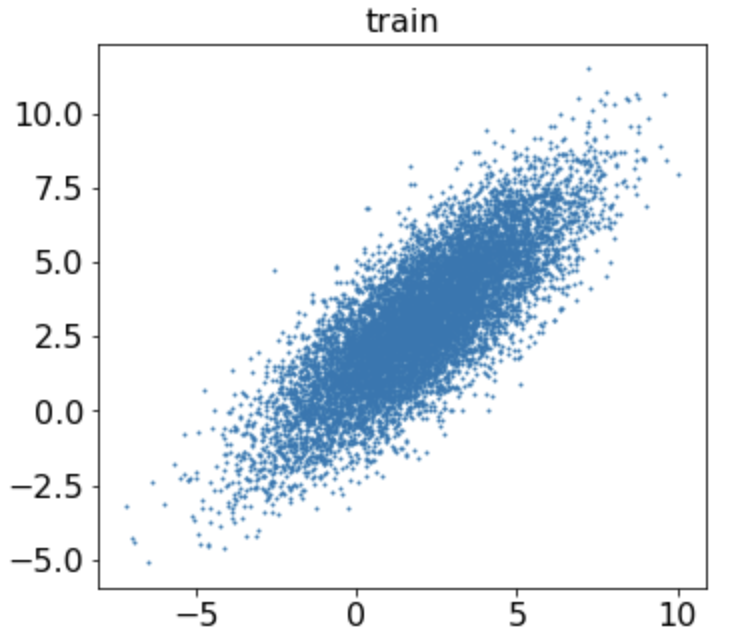
\includegraphics[width=.8\linewidth]{figs/posterior_collapse_toy_1.png}
			\end{figure}
		\end{minipage}%
		\begin{minipage}[t]{0.33\columnwidth}
			\begin{figure}[h]
				\centering
				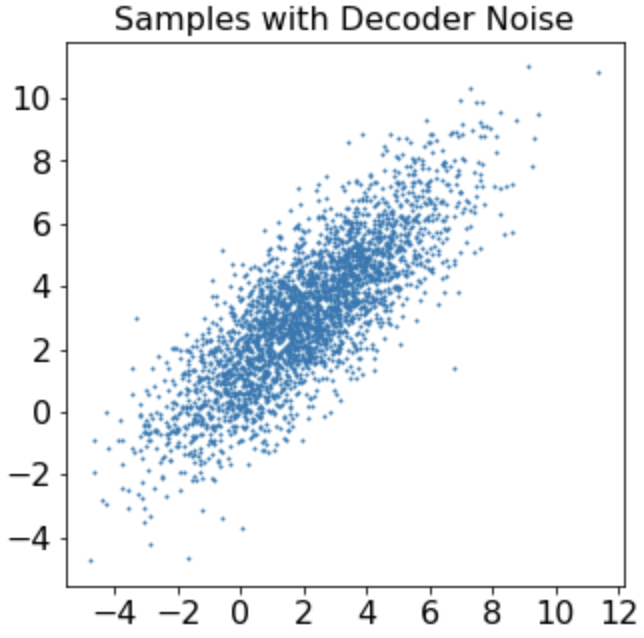
\includegraphics[width=0.75\linewidth]{figs/posterior_collapse_toy_3.png}
			\end{figure}
		\end{minipage}%
		\begin{minipage}[t]{0.33\columnwidth}
			\begin{figure}[h]
				\centering
				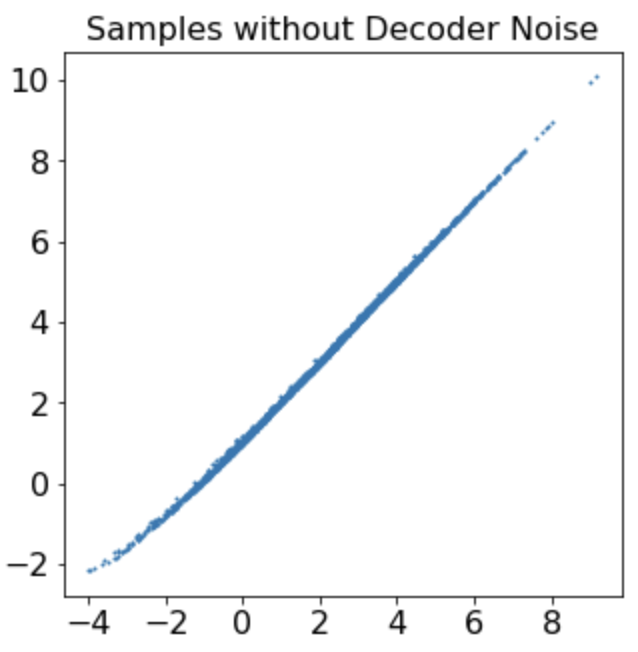
\includegraphics[width=.75\linewidth]{figs/posterior_collapse_toy_5.png}
			\end{figure}
		\end{minipage}
	The encoder uses latent variables to model data.
	\end{block}

	\begin{block}{Univariate ($\bSigma$ is diagonal)}
		\vspace{-0.5cm}
		\begin{minipage}[t]{0.33\columnwidth}
		\begin{figure}[h]
			\centering
			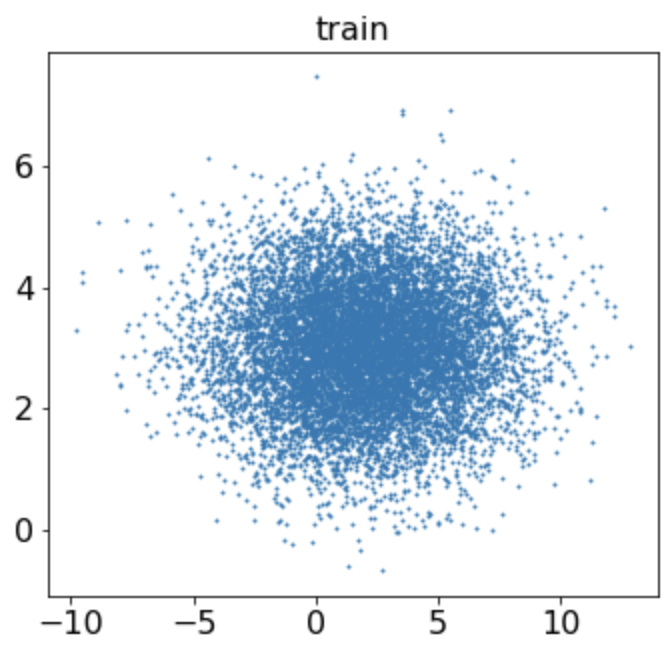
\includegraphics[width=.8\linewidth]{figs/posterior_collapse_toy_2.png}
		\end{figure}
		\end{minipage}%
		\begin{minipage}[t]{0.33\columnwidth}
		\begin{figure}[h]
			\centering
			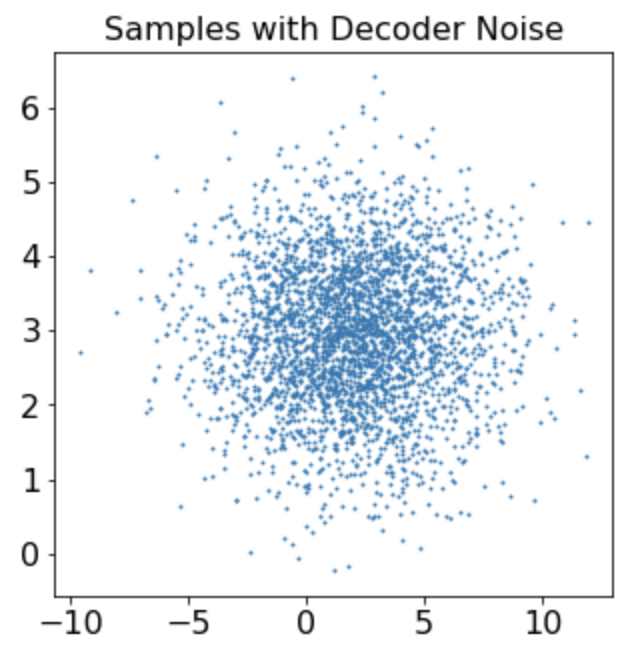
\includegraphics[width=.75\linewidth]{figs/posterior_collapse_toy_4.png}
		\end{figure}
		\end{minipage}%
		\begin{minipage}[t]{0.33\columnwidth}
		\begin{figure}[h]
			\centering
			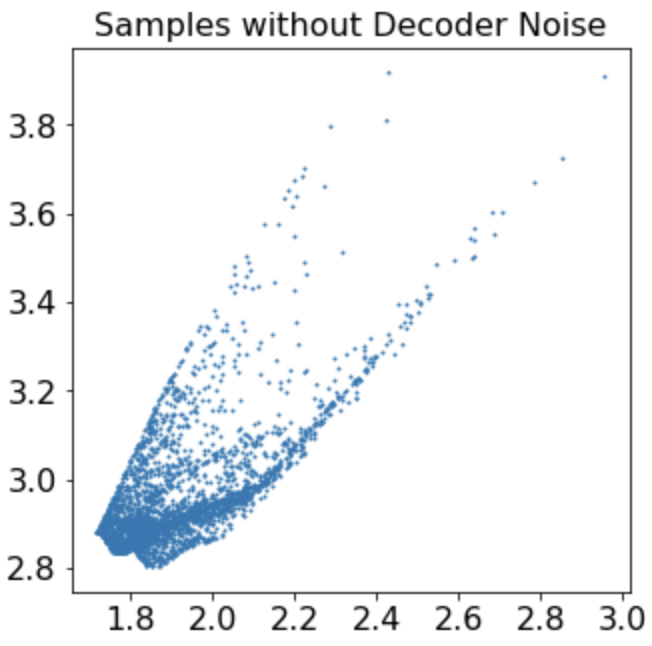
\includegraphics[width=.75\linewidth]{figs/posterior_collapse_toy_6.png}
		\end{figure}
		\end{minipage}
	Latent variables are not used, since the decoder could model the data without the encoder.
	\end{block}
\end{frame}
%=======
\begin{frame}{Posterior collapse}
	\begin{block}{Representation learning}
		"Identifies and disentangles the underlying causal factors of the data, so that it becomes easier to understand the data, to classify it, or to perform other tasks".
	\end{block}
	\[
		p(\bx | \btheta) = \int p(\bx, \bz | \btheta) d \bz = \int p(\bx | \bz, \btheta) p(\bz) d \bz 
	\]
	If the decoder model $p(\bx | \bz, \btheta)$ is powerful enough to model $p(\bx | \btheta)$ the latent variables $\bz$ becames irrelevant.
	
	\[
		\mathcal{L}(q, \btheta) = \frac{1}{n} \sum_{i=1}^n \left[ \mathbb{E}_{q(\bz_i | \bx_i)} \log p(\bx_i | \bz_i, \btheta) - KL(q(\bz_i | \bx_i) || p(\bz_i)) \right].
	\]
	Early in the training the approximate posterior $q(\bz|\bx)$ carries little information about $\bx$ and the model sets the posterior to the prior to avoid paying any cost $KL(q(\bz|\bx)||p(\bz))$.
\end{frame}
%=======
\begin{frame}{PixelVAE}
	\[
	    p(\bx | \btheta) = \int p(\bx, \bz | \btheta) d \bz = \int p(\bx | \bz, \btheta) p(\bz) d \bz 
	\]
	\begin{itemize}
		\item More powerful $p(\bx | \bz, \btheta)$ leads to more powerful generative model $p(\bx | \btheta)$.
		\item Too powerful $p(\bx | \bz, \btheta)$ could lead to posterior collapse, where variational posterior $q(\bz | \bx)$ will not carry any information about data and close to prior $p(\bz)$.
	\end{itemize}
	How to make the generative model $p(\bx | \bz, \btheta)$ more powerful?
	\begin{block}{Autoregressive decoder}
	\[
	    p(\bx | \bz , \btheta) = \prod_{i=1}^n p(x_i | \bx_{1:i - 1}, \bz , \btheta)
	\]
	\end{block}
	
	\myfootnotewithlink{https://arxiv.org/abs/1611.05013}{Gulrajani I. et al. PixelVAE: A Latent Variable Model for Natural Images, 2016}
\end{frame}
%=======
\begin{frame}{PixelVAE}
	VAE model with autoregressive PixelCNN decoder with few autoregressive layers. 
	\begin{itemize}
		\item Global structure is captured by latent variables.
		\item Local statistics are captured by limited receptive field autoregressive model.
	\end{itemize}
	\begin{figure}
	    \centering
	    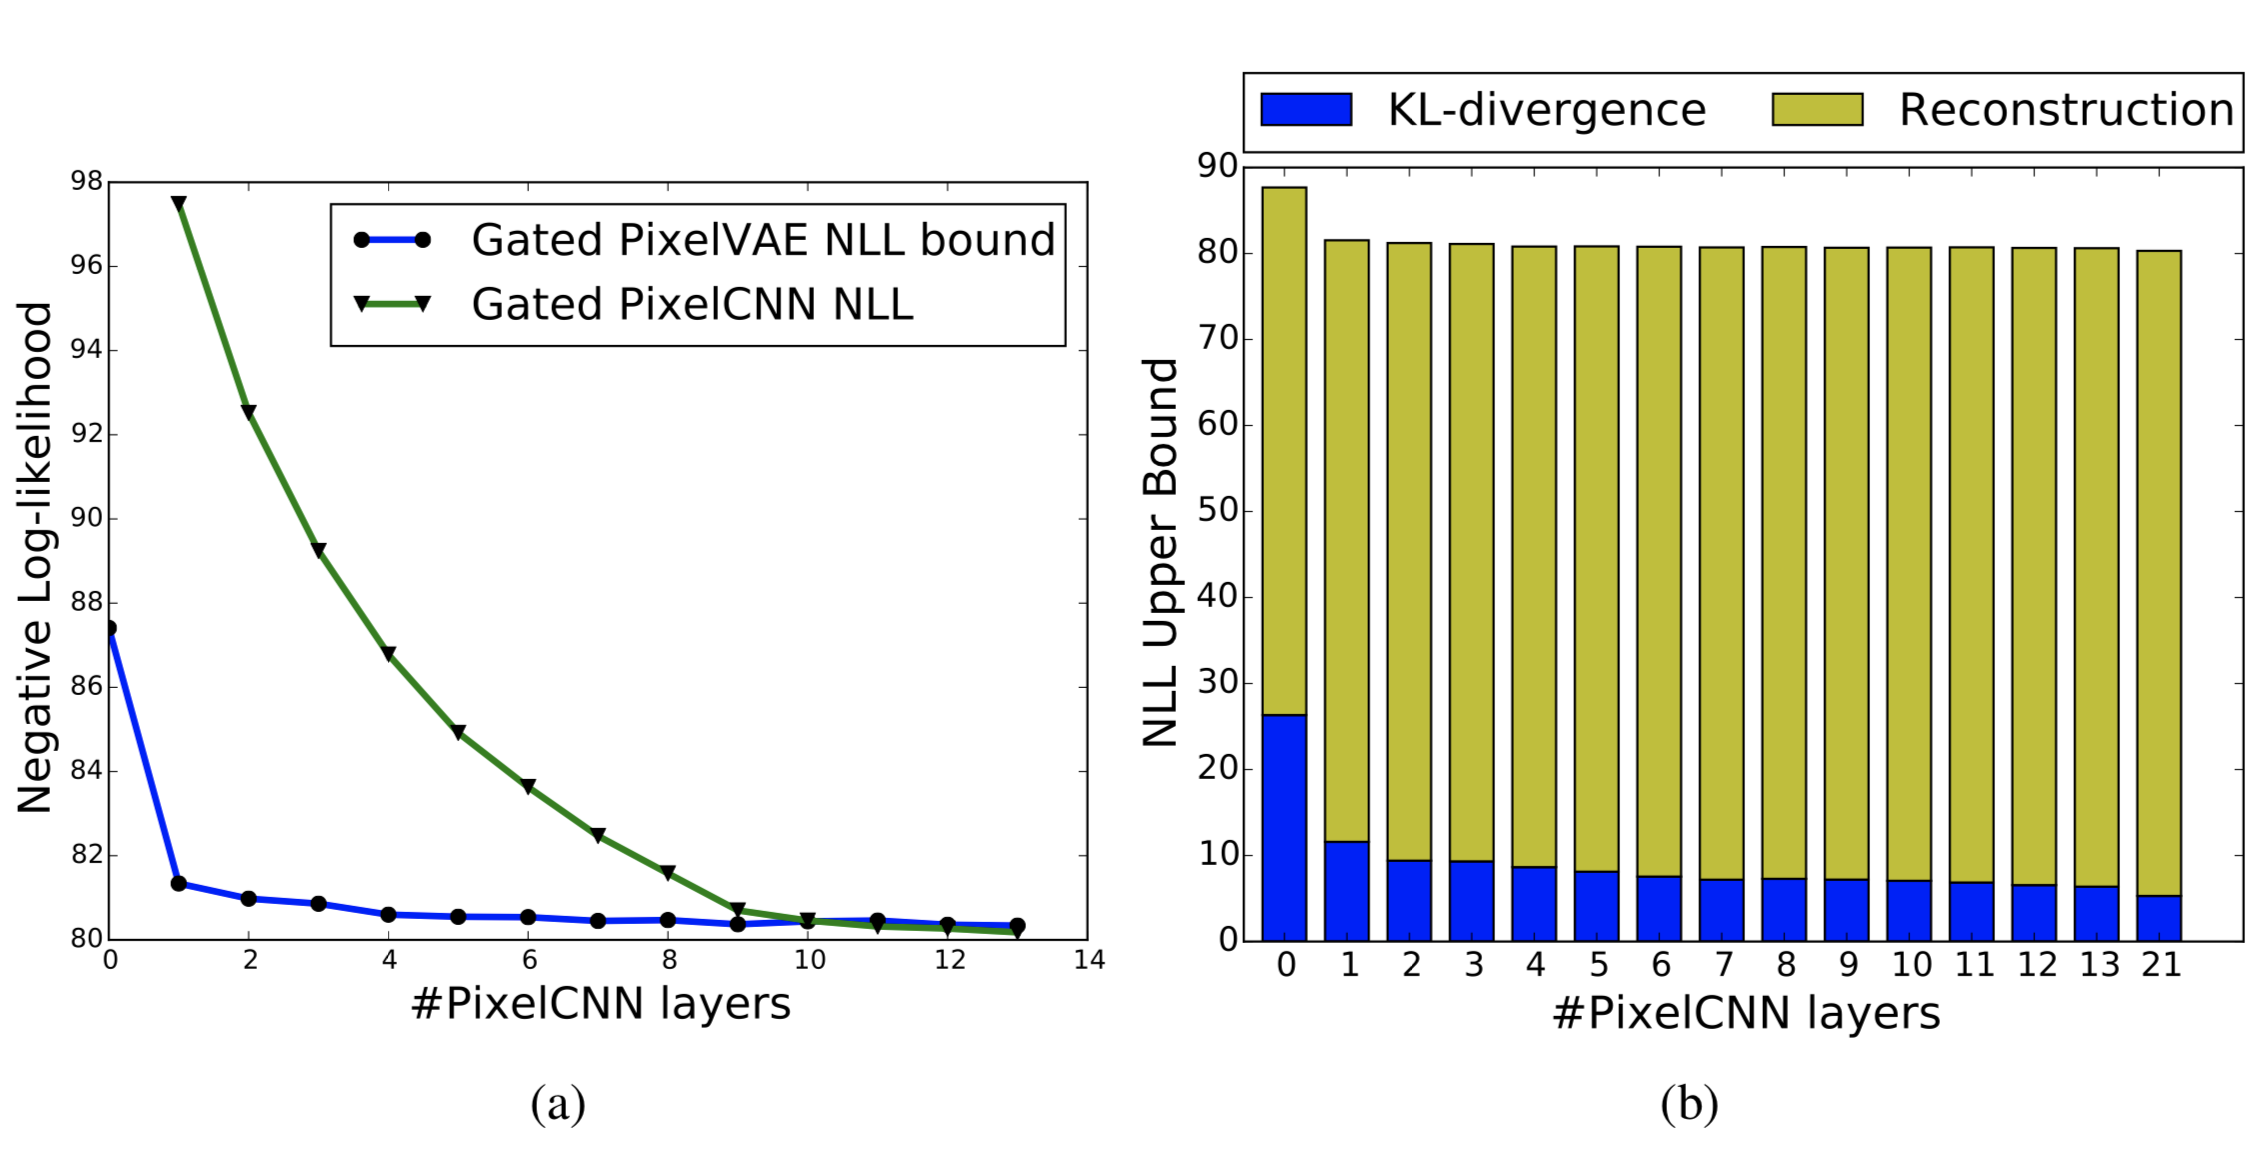
\includegraphics[width=0.8\linewidth]{figs/PixelVAE_2.png}
	\end{figure}
		
	\myfootnotewithlink{https://arxiv.org/abs/1611.05013}{Gulrajani I. et al. PixelVAE: A Latent Variable Model for Natural Images, 2016}
\end{frame}
%=======
\begin{frame}{PixelVAE}
	\begin{minipage}[t]{0.5\columnwidth}
		MNIST
		\begin{figure}
			\centering
			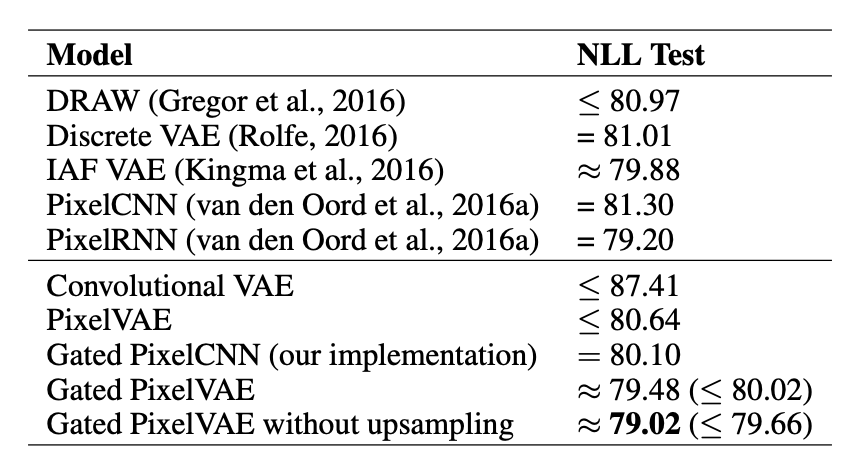
\includegraphics[width=0.9\linewidth]{figs/PixelVAE_5.png}
		\end{figure}
	\end{minipage}%
	\begin{minipage}[t]{0.5\columnwidth}
		ImageNet 64x64
		\begin{figure}
			\centering
			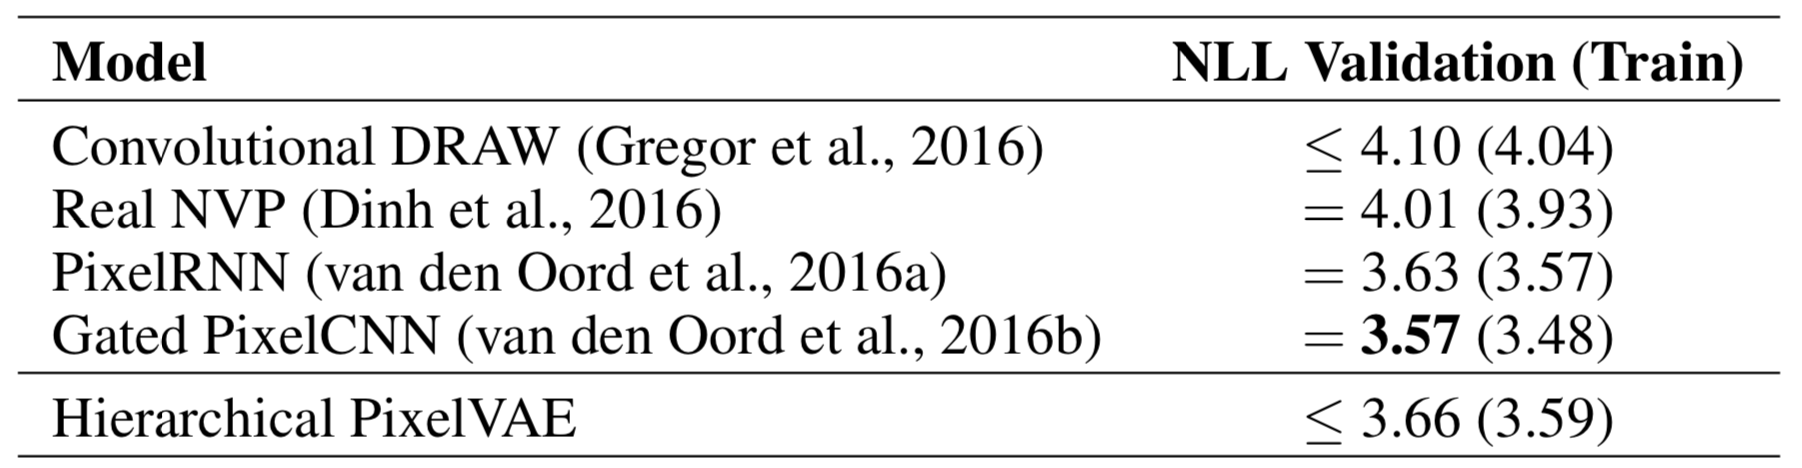
\includegraphics[width=\linewidth]{figs/PixelVAE_4.png}
		\end{figure}
	\end{minipage}
	\begin{figure}
	    \centering
	    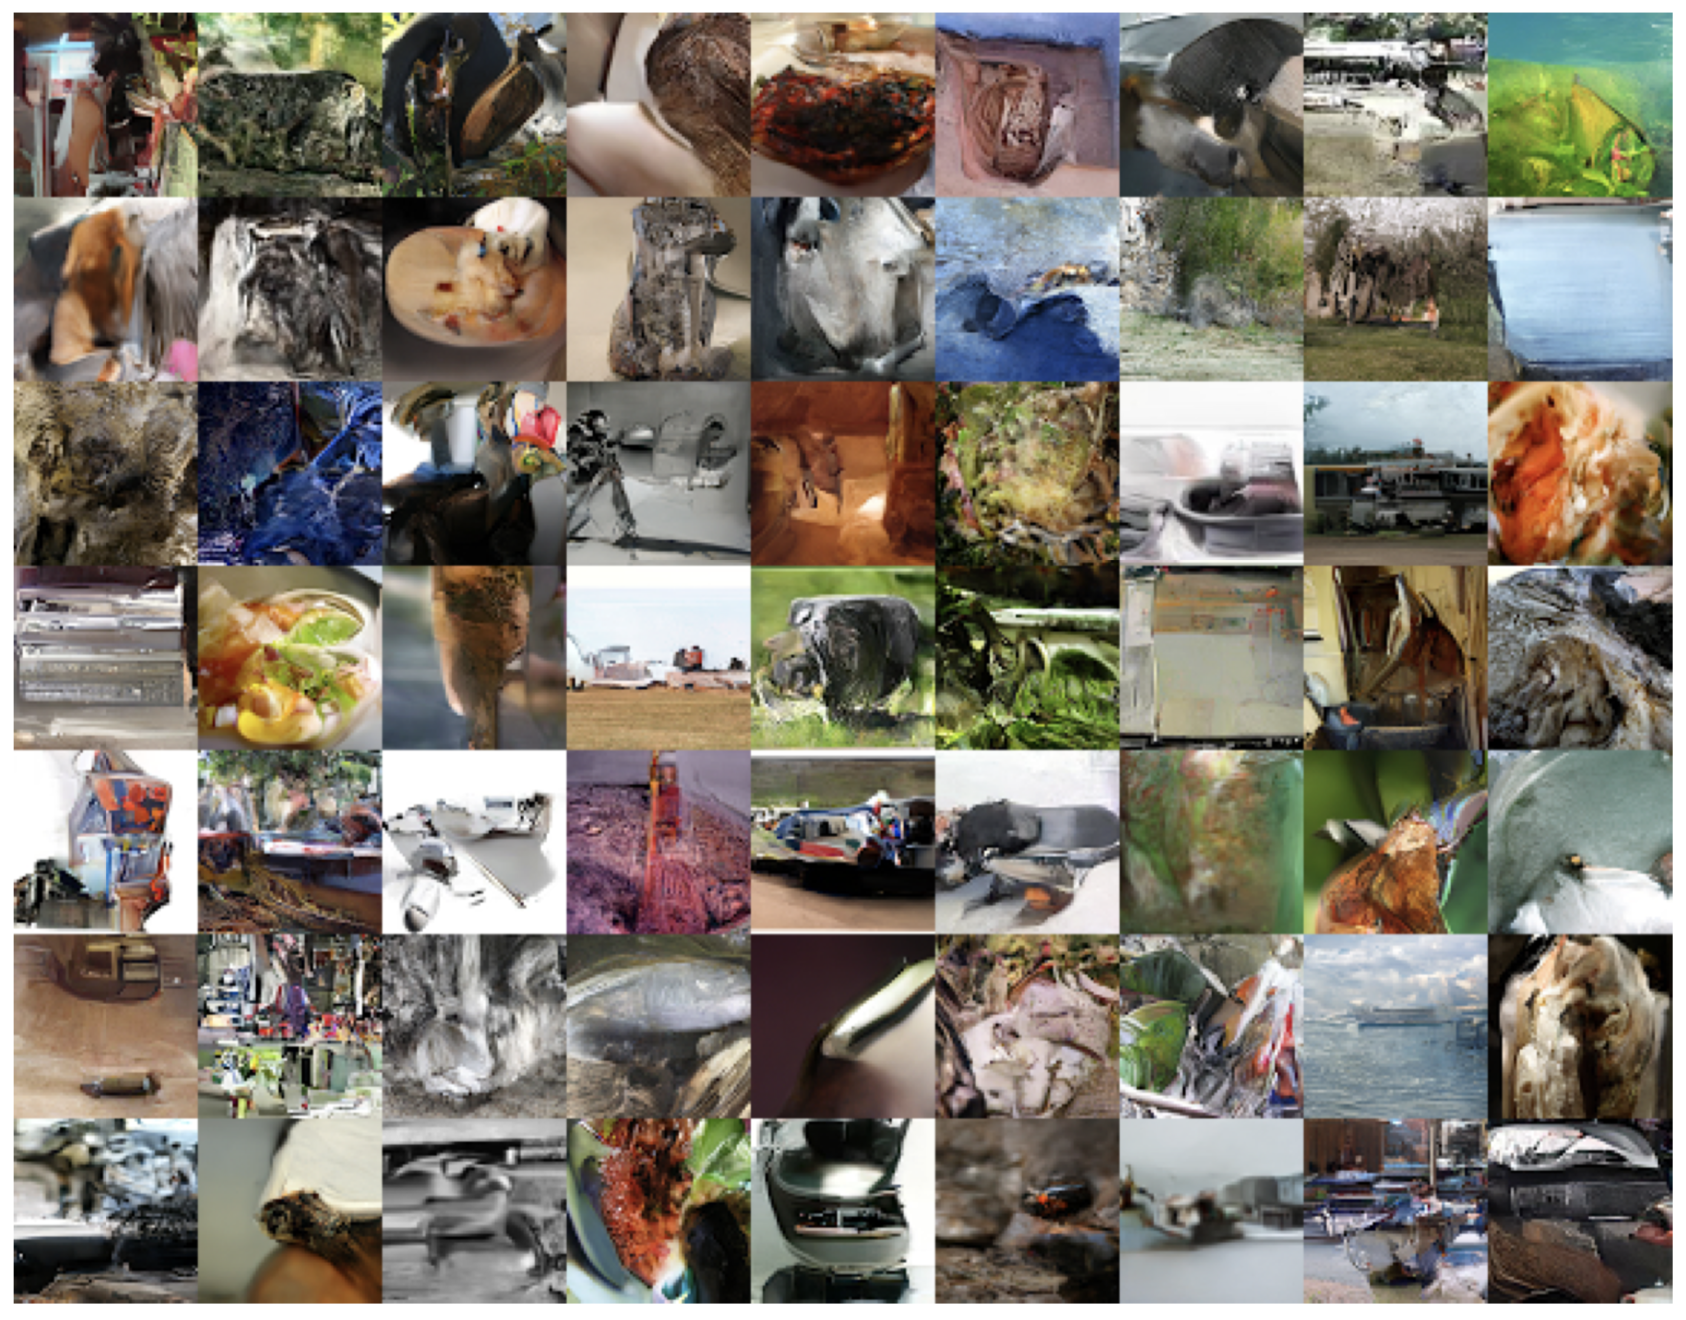
\includegraphics[width=0.5\linewidth]{figs/PixelVAE_3.png}
	\end{figure}
	
	\myfootnotewithlink{https://arxiv.org/abs/1611.05013}{Gulrajani I. et al. PixelVAE: A Latent Variable Model for Natural Images, 2016}
\end{frame}
%=======
\begin{frame}{Decoder weakening}
	\[
		p(\bx | \btheta) = \int p(\bx, \bz | \btheta) d \bz = \int p(\bx | \bz, \btheta) p(\bz) d \bz 
	\]
	Powerful decoder $p(\bx | \bz, \btheta)$ makes the model expressive, but posterior collapse is possible.
	
	PixelVAE model uses the autoregressive PixelCNN model with small number of layers to limit receptive field.
	
	How to force the model encode information about $\bx$ into $\bz$?
	\[
	    \mathcal{L}(q, \btheta) = \mathbb{E}_{q(\bz | \bx)} \log p(\bx | \bz, \btheta) - \beta \cdot KL (q(\bz | \bx) || p(\bz))
	\]
	What we get if $\beta = 1$ ($\beta = 0$)? \\
	
	\begin{block}{KL annealing}
		\begin{itemize}
		    \item Start training with $\beta = 0$.
		    \item Increase it until $\beta = 1$ during training process.
		\end{itemize}
	\end{block}
	\myfootnotewithlink{https://arxiv.org/abs/1511.06349}{Bowman S. R. et al. Generating Sentences from a Continuous Space, 2015}
\end{frame}
%=======
\begin{frame}{Decoder weakening}
	\begin{block}{Free bits}
	\begin{itemize}
	\item Divide the latent dimensions into the $K$ subsets.
	\item Ensure the use of less than $\lambda$ nats of information per subset $j$.
	\end{itemize}
	
	\[
	    \hat{\mathcal{L}}(q, \btheta) = \mathbb{E}_{q(\bZ | \bX)} \log p(\bX | \bZ, \btheta) - \sum_{j=1}^K \max(\lambda, KL (q(\bZ_j | \bX) || p(\bZ_j))).
	\]
	
	Increasing the latent information is advantageous for the reconstruction term. \\
	\vspace{0.2cm}
	This results in $KL (q(\bZ_j | \bx) || p(\bZ_j)) \geq \lambda$ for all $j$, in practice.
	\end{block}
	\myfootnotewithlink{https://arxiv.org/abs/1606.04934}{Kingma D. P. et al. Improving Variational Inference with Inverse Autoregressive Flow, 2016}
\end{frame}
%=======
\begin{frame}{Variational Lossy AutoEncoder, 2016}
	\begin{block}{Lossy code via explicit information placement}
	\[
	    p(\bx | \bz, \btheta) = \prod_{i=1}^m p(x_i | \bz, \bx_{\text{WindowAround}(i)}, \btheta).
	\]
	\begin{itemize}
	    \item WindowAround($i$) restricts the receptive field (it forbids to represent arbitrarily complex distribution over $\bx$ without dependence on $\bz$). 
	    \item Local statistics of 2D images (texture) will be modeled by a small local window.
	    \item Global structural information (shapes) is long-range dependency that can only be communicated through latent code $\bz$. 
	\end{itemize}
	\end{block}
	\myfootnotewithlink{https://arxiv.org/abs/1611.02731}{Chen X. et al. Variational Lossy Autoencoder, 2016}
\end{frame}
%=======
\begin{frame}{Variational Lossy AutoEncoder, 2016}
\begin{itemize}
    \item Can VLAE learn lossy codes that encode global statistics?
    \item Does using AF priors improves upon using IAF posteriors as predicted by theory?
    \item Does using autoregressive decoding distributions improve density estimation performance?
\end{itemize}
	\begin{minipage}[t]{0.5\columnwidth}
	\vspace{1cm}
		MNIST
		\begin{figure}[h]
			\centering
			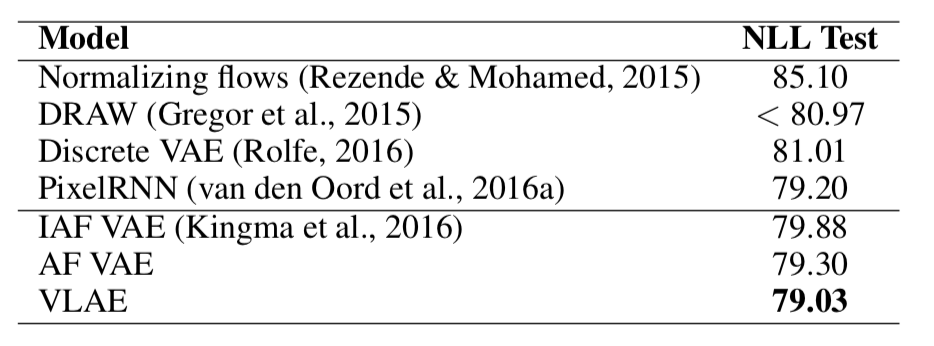
\includegraphics[width=1.\linewidth]{figs/VLAE_1.png}
		\end{figure}
	\end{minipage}%
	\begin{minipage}[t]{0.5\columnwidth}
		CIFAR10
		\begin{figure}[h]
			\centering
			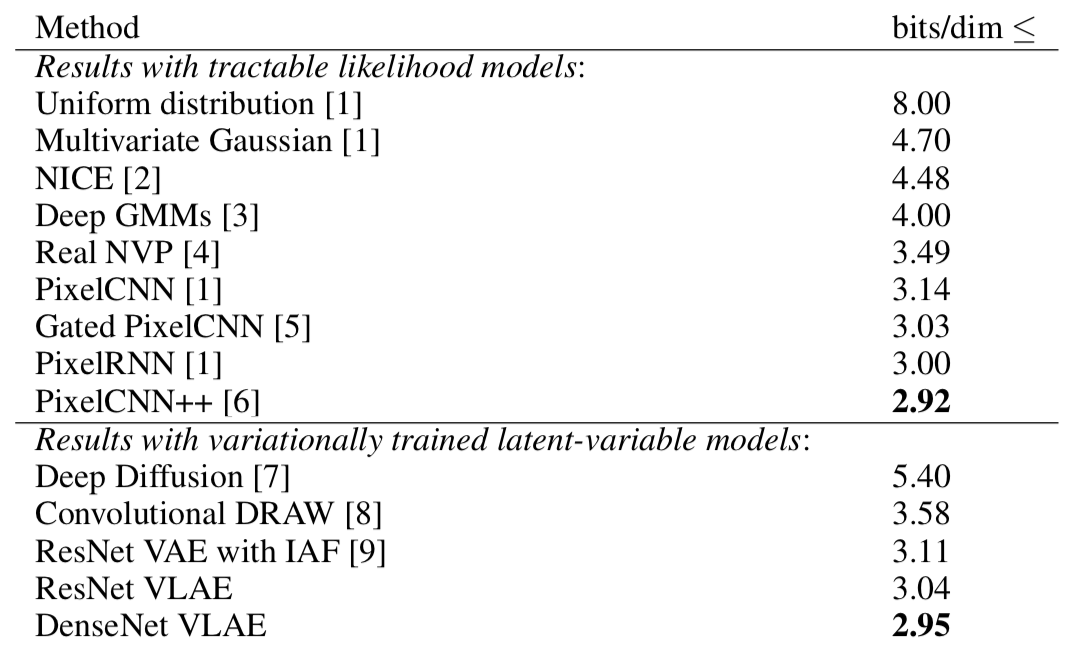
\includegraphics[width=1.\linewidth]{figs/VLAE_2.png}
		\end{figure}
	\end{minipage}

	\myfootnotewithlink{https://arxiv.org/abs/1611.02731}{Chen X. et al. Variational Lossy Autoencoder, 2016}
\end{frame}
%=======
\begin{frame}{Disentangled representations}
	\begin{block}{Unsupervised representation learning}
	    Learning an interpretable factorised representation of the independent data generative factors of the world without supervision. 
	\end{block}
	\begin{block}{Disentanglement informal definition}
	A disentangled representation can be defined as one where single latent units are sensitive to changes in single generative factors, while being relatively invariant to changes in other factors. 
	\end{block}
	\begin{block}{Example}
	Model trained on a dataset of 3D objects might learn independent latent units sensitive to single independent data generative factors, such as object identity, position, scale, lighting or colour. 
	\end{block}
	\myfootnotewithlink{https://openreview.net/references/pdf?id=Sy2fzU9gl}{Higgins I. et al. beta-VAE: Learning Basic Visual Concepts with a Constrained Variational Framework, 2017}
\end{frame}
%=======
\begin{frame}{$\beta$-VAE, 2017}
	\begin{block}{Generative process}
	\begin{itemize}
	    \item $p(\bx | \bv, \bw) = \text{Sim}(\bv, \bw)$~-- true world simulator;
	    \item $\bv$~-- conditionally independent factors: $p(\bv | \bx) = \prod_{j=1}^d p(v_j | \bx)$;
	    \item $\bw$~-- conditionally dependent factors. 
	\end{itemize}
	\end{block}
	\begin{block}{Goal}
	Construct an unsupervised deep generative model
	\[
	    p(\bx | \bz) \approx p(\bx | \bv, \bw).
	\]
	\vspace{-0.5cm}
	\begin{itemize}
	    \item Ensure that the inferred latent factors $q(\bz|\bx)$ capture the factors $\bv$ in a disentangled manner. 
	    \item The conditionally dependent factors $\bw$ can remain entangled in a separate subset of $\bz$ that is not used for representing $\bv$. 
	\end{itemize}
	\end{block}
	\myfootnotewithlink{https://openreview.net/references/pdf?id=Sy2fzU9gl}{Higgins I. et al. beta-VAE: Learning Basic Visual Concepts with a Constrained Variational Framework, 2017}
\end{frame}
%=======
\begin{frame}{$\beta$-VAE}
	\vspace{-0.5cm}
	\begin{block}{Constrained optimization}
	\vspace{-0.5cm}
	\[
	    \max_{q, \btheta} \mathbb{E}_{q(\bz | \bx)} \log p(\bx | \bz, \btheta), \quad \text{subject to } KL (q(\bz | \bx) || p(\bz)) < \epsilon.
	\]
	\vspace{-0.7cm}
	\end{block}
	\begin{block}{Objective}
	\vspace{-0.5cm}
	\[
	    \mathcal{L}(q, \btheta, \beta) = \mathbb{E}_{q(\bz | \bx)} \log p(\bx | \bz, \btheta) - \beta \cdot KL (q(\bz | \bx) || p(\bz)).
	\]
	\vspace{-0.5cm}
	\end{block}
	What do we get at $\beta = 1$? \\
	\begin{block}{Hypothesis}
	To learn disentangled representations of the conditionally independent factors $\bv$, it is important to set a stronger constraint on the latent bottleneck: $\beta > 1$.
	\end{block}
	\textbf{Note:} It leads to poorer reconstructions and a loss of high frequency details when passing through a constrained latent bottleneck. 
	\myfootnotewithlink{https://openreview.net/references/pdf?id=Sy2fzU9gl}{Higgins I. et al. beta-VAE: Learning Basic Visual Concepts with a Constrained Variational Framework, 2017}
\end{frame}
%=======
\begin{frame}{$\beta$-VAE}
	\begin{block}{Disentangling metric}
		\begin{enumerate}
			\item Generate two sets of objects
			\[
			\bx_{li} \sim \text{Sim}(\bv_{li}, \bw_{li}); \quad \bx_{lj} \sim \text{Sim}(\bv_{lj}, \bw_{lj}); \quad y_{ij} \sim U[1, d].
			\]
			\[
			\bv_{li} \sim p(\bv); \quad \bv_{lj} \sim p(\bv) \, ([v_{li}]_y = [v_{lj}]_y); \quad \bw_{li}, \bw_{lj} \sim p(\bw).
			\]
			\item Find representations
			\[
			q(\bz | \bx) = \mathcal{N}\left(\mu(\bx) | \sigma^2(\bx)\right); \quad \bz_{li} = \mu(\bx_{li}); \quad \bz_{lj} = \mu(\bx_{lj}).
			\]
			\item Use accuracy of classifier $p(y | \bz_{\text{diff}})$ with a low VC-dimension as metric of disentanglement
			\[
			\bz_{\text{diff}} = \frac{1}{L} \sum_{l=1}^L | \bz_{li} - \bz_{lj} |.
			\]
		\end{enumerate}
	
	\end{block}
	\myfootnotewithlink{https://openreview.net/references/pdf?id=Sy2fzU9gl}{Higgins I. et al. beta-VAE: Learning Basic Visual Concepts with a Constrained Variational Framework, 2017}
\end{frame}
%=======
\begin{frame}{$\beta$-VAE}
	\begin{figure}
	    \centering
	    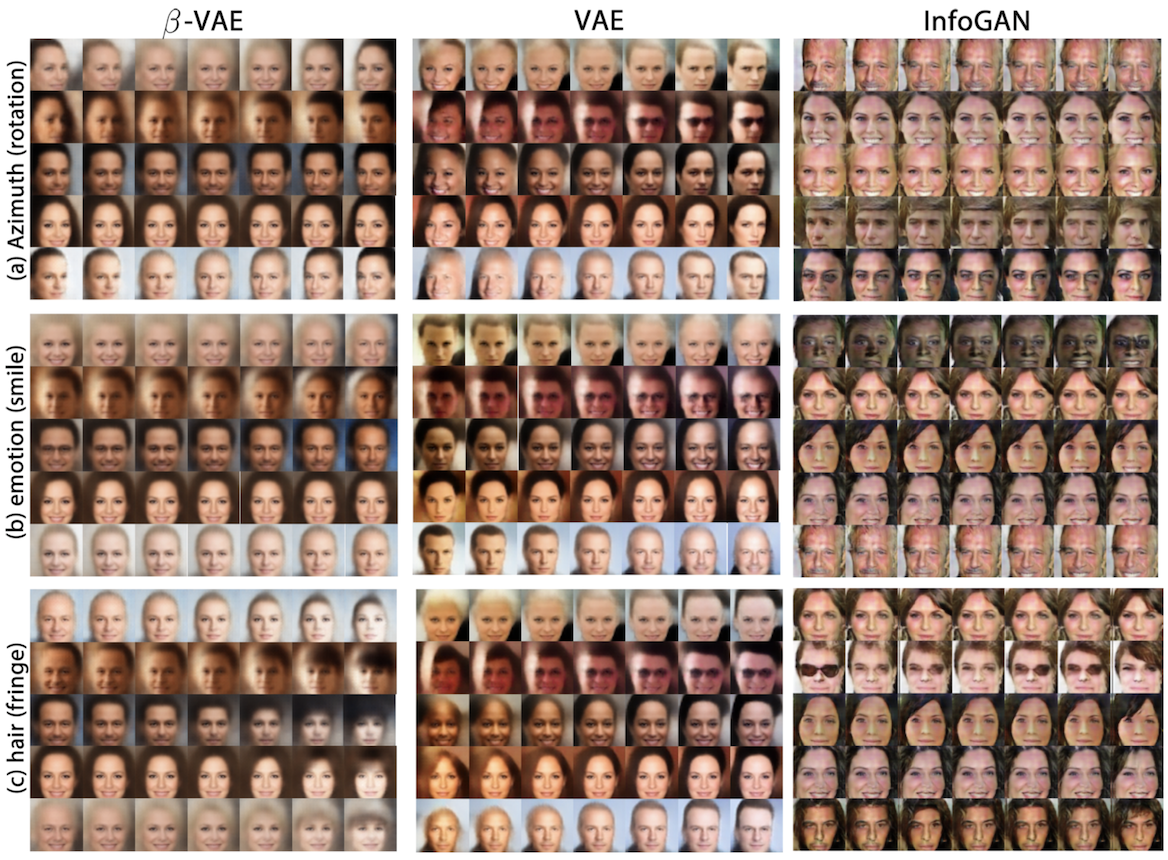
\includegraphics[width=0.95\linewidth]{figs/betaVAE_1.png}
	\end{figure}

	\myfootnotewithlink{https://openreview.net/references/pdf?id=Sy2fzU9gl}{Higgins I. et al. beta-VAE: Learning Basic Visual Concepts with a Constrained Variational Framework, 2017}
\end{frame}
%=======
\begin{frame}{$\beta$-VAE}
	\vspace{1cm}
	\begin{figure}
	    \centering
	    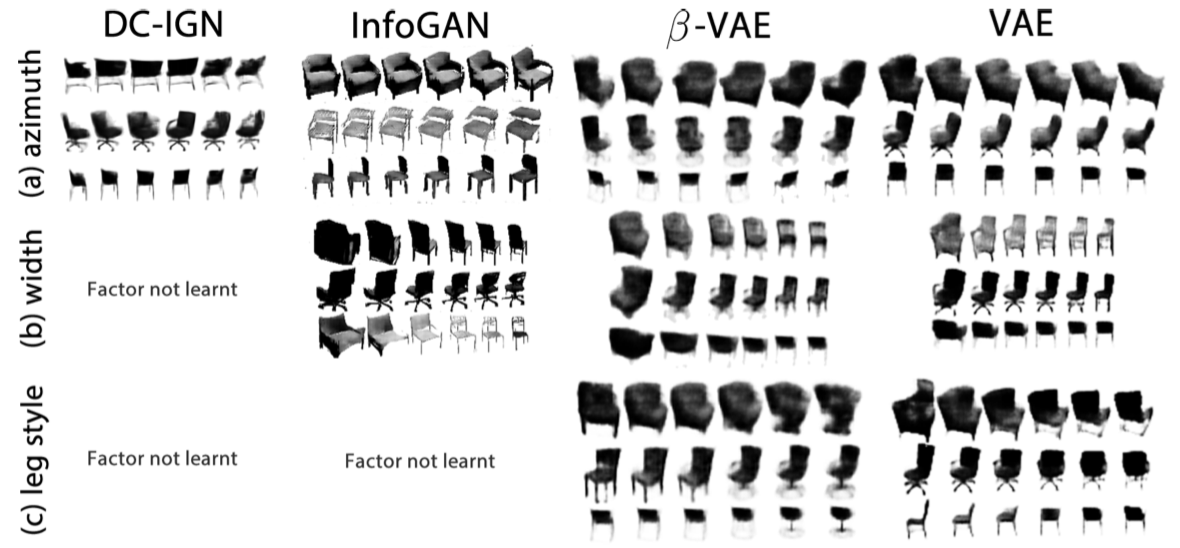
\includegraphics[width=\linewidth]{figs/betaVAE_2.png}
	\end{figure}

	\myfootnotewithlink{https://openreview.net/references/pdf?id=Sy2fzU9gl}{Higgins I. et al. beta-VAE: Learning Basic Visual Concepts with a Constrained Variational Framework, 2017}
\end{frame}
%=======
\begin{frame}{$\beta$-VAE}
	\begin{figure}
	    \centering
	    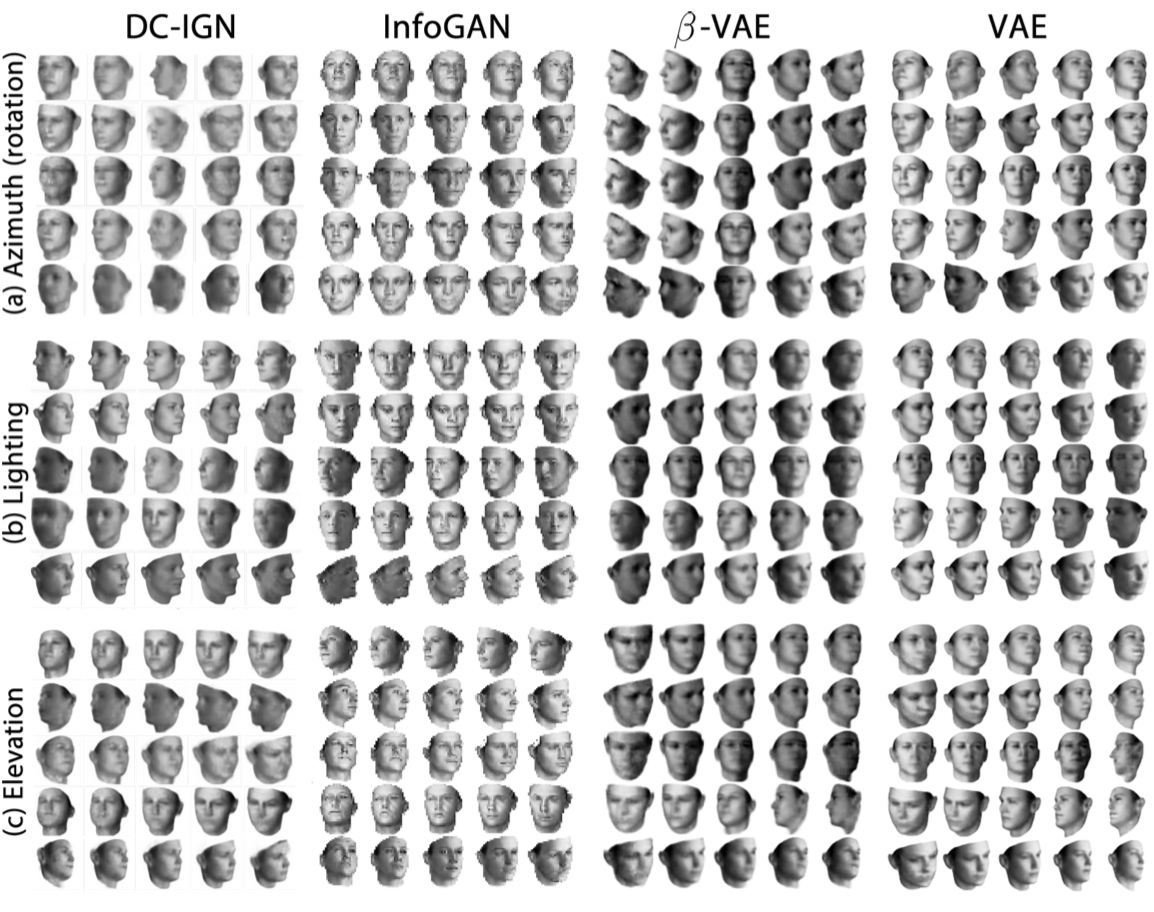
\includegraphics[width=0.8\linewidth]{figs/betaVAE_3.png}
	\end{figure}

	\myfootnotewithlink{https://openreview.net/references/pdf?id=Sy2fzU9gl}{Higgins I. et al. beta-VAE: Learning Basic Visual Concepts with a Constrained Variational Framework, 2017}
\end{frame}
%=======
\begin{frame}{$\beta$-VAE}
	\begin{minipage}[t]{0.5\columnwidth}
	    \vspace{1.5cm}
		\begin{figure}
			\centering
			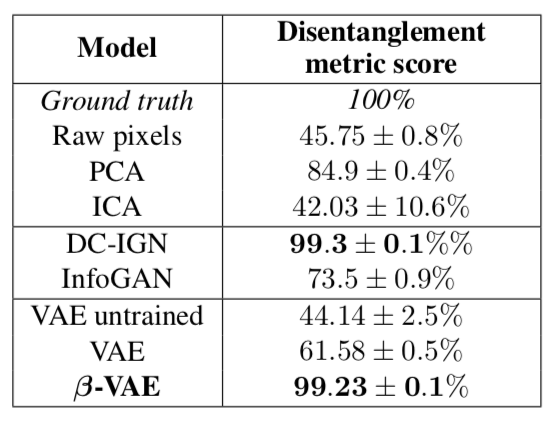
\includegraphics[width=1.\linewidth]{figs/betaVAE_4.png}
		\end{figure}
	\end{minipage}%
	\begin{minipage}[t]{0.5\columnwidth}
		\begin{figure}[h]
			\centering
			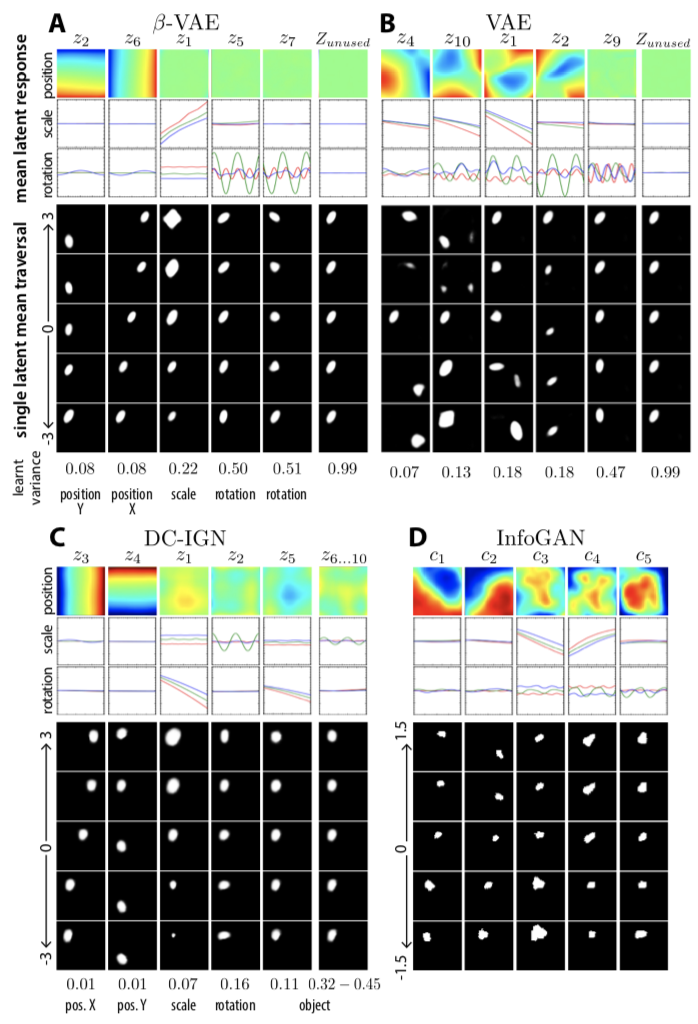
\includegraphics[width=.95\linewidth]{figs/betaVAE_5.png}
		\end{figure}
	\end{minipage}

	\myfootnotewithlink{https://openreview.net/references/pdf?id=Sy2fzU9gl}{Higgins I. et al. beta-VAE: Learning Basic Visual Concepts with a Constrained Variational Framework, 2017}
\end{frame}
%=======
\begin{frame}{$\beta$-VAE}
	\begin{itemize}
		\item \textbf{Top row:} original images.
		\item \textbf{Second row:} the corresponding reconstructions. 
		\item \textbf{Remaining rows:} latent traversals ordered by KL divergence with the prior. 
		\item \textbf{Heatmaps:} latent activations for each 2D position.
	\end{itemize}
	\begin{figure}
	    \centering
	    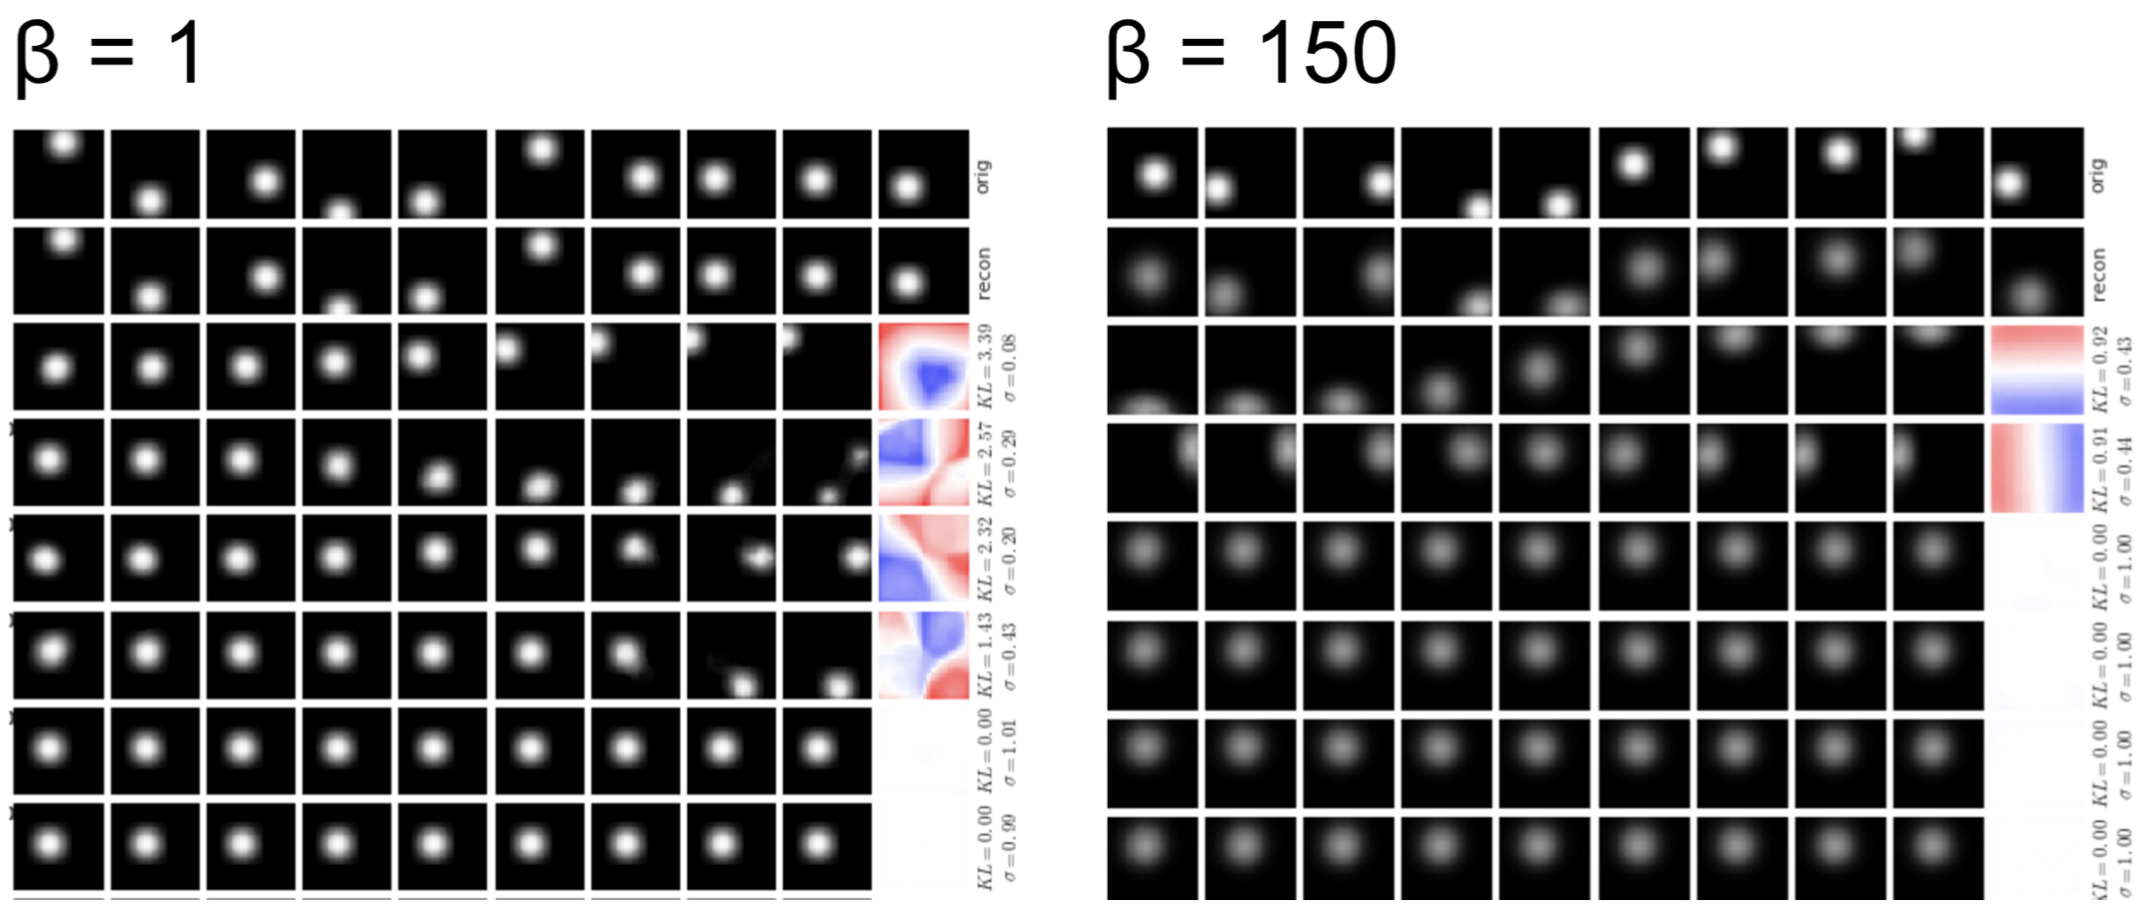
\includegraphics[width=\linewidth]{figs/betaVAE_6.png}
	\end{figure}
	\myfootnotewithlink{https://arxiv.org/abs/1804.03599}{Burgess C. P. et al. Understanding disentangling in $\beta$-VAE, 2018}
\end{frame}
%=======
\begin{frame}{$\beta$-VAE}
	\begin{block}{Controlled encoding capacity}
	\vspace{-0.5cm}
	\[
	    \mathcal{L}(q, \btheta, \beta) = \mathbb{E}_{q(\bz | \bx)} \log p(\bx | \bz, \btheta) - | KL (q(\bz | \bx) || p(\bz)) - C|.
	\]
	\end{block}
	\begin{figure}
	    \centering
	    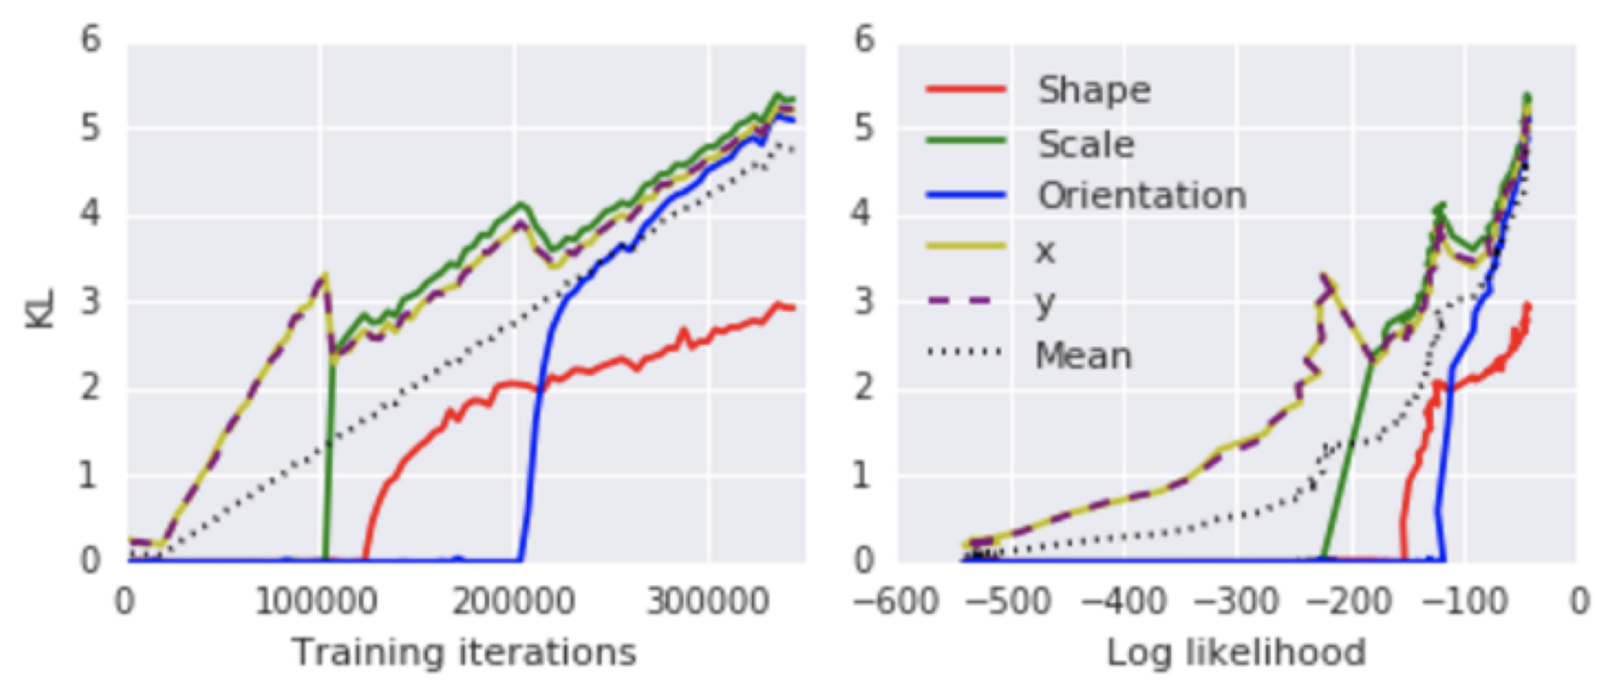
\includegraphics[width=0.9\linewidth]{figs/betaVAE_7.png}
	\end{figure}
	The early capacity is allocated to positional latents only, followed by a scale latent, then shape and orientation latents.

	\myfootnotewithlink{https://arxiv.org/abs/1804.03599}{Burgess C. P. et al. Understanding disentangling in $\beta$-VAE, 2018}
\end{frame}
%=======
\begin{frame}{$\beta$-VAE}
	\begin{block}{Controlled encoding capacity}
	\vspace{-0.5cm}
	\[
	    \mathcal{L}(q, \btheta, \beta) = \mathbb{E}_{q(\bz | \bx)} \log p(\bx | \bz, \btheta) - | KL (q(\bz | \bx) || p(\bz)) - C|.
	\]
	\vspace{-0.5cm}
	\end{block}
	\begin{figure}
	    \centering
	    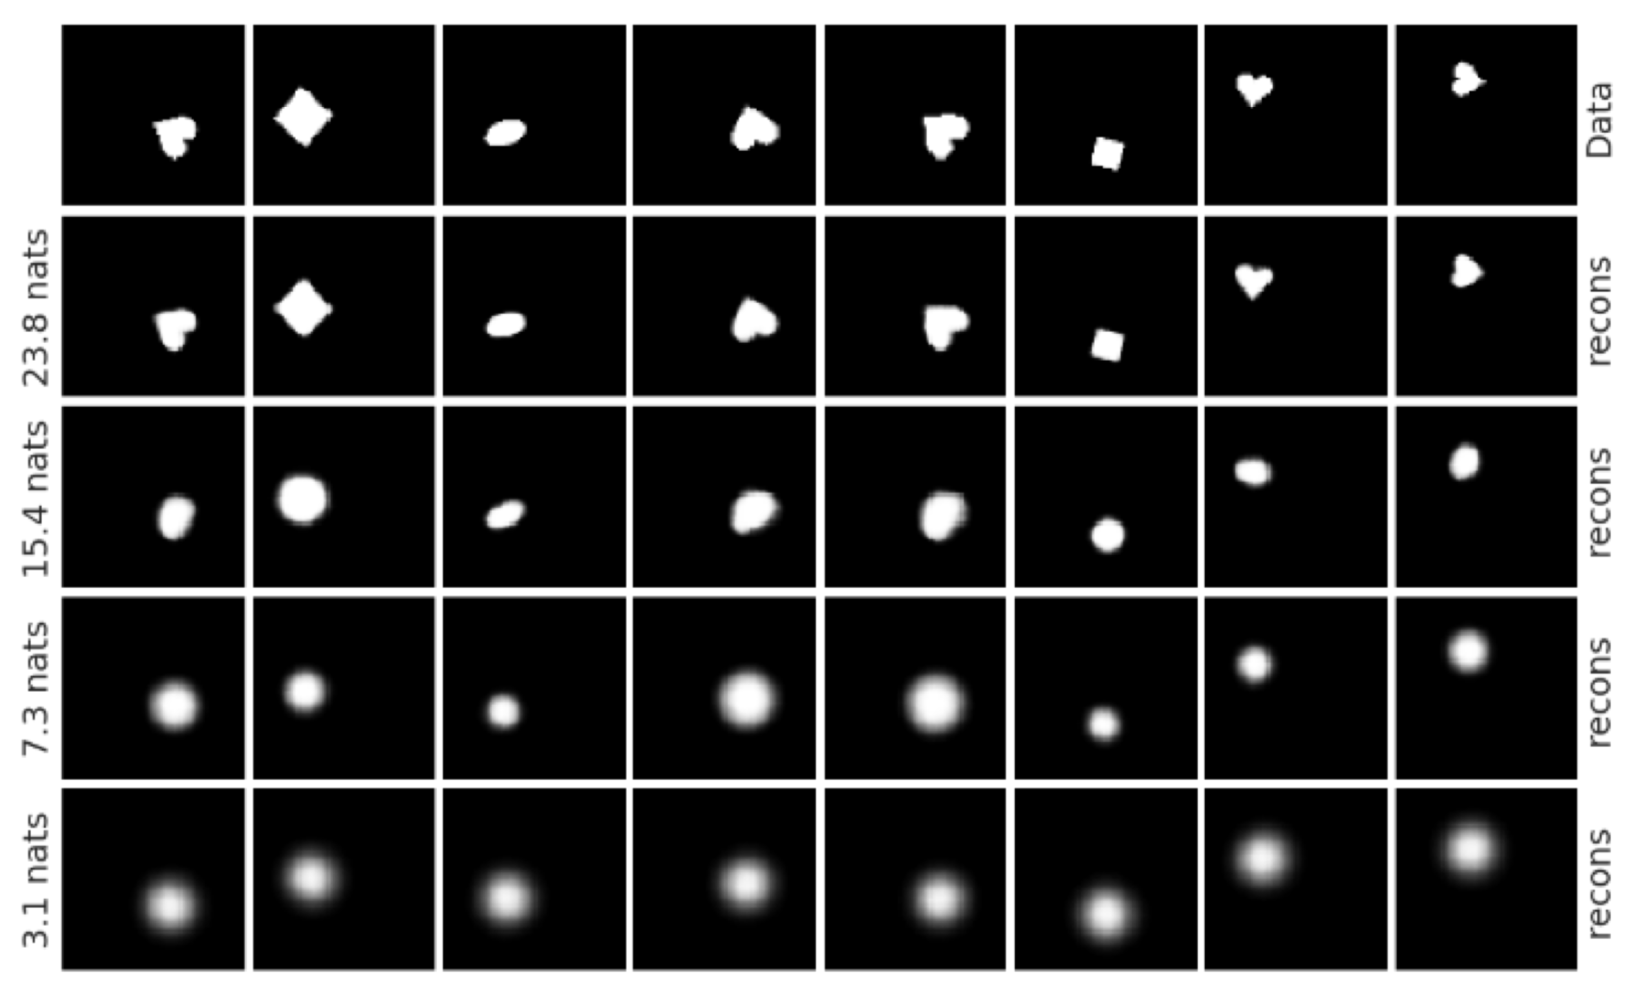
\includegraphics[width=0.7\linewidth]{figs/betaVAE_8.png}
	\end{figure}
	As the information capacity increases the different latents associated with their data generative factors become informative.

	\myfootnotewithlink{https://arxiv.org/abs/1804.03599}{Burgess C. P. et al. Understanding disentangling in $\beta$-VAE, 2018}
\end{frame}
%=======
\begin{frame}{$\beta$-VAE}
	\begin{block}{Single latent traversals, ordered by their average KL divergence with the prior}
		\begin{figure}
		\centering
		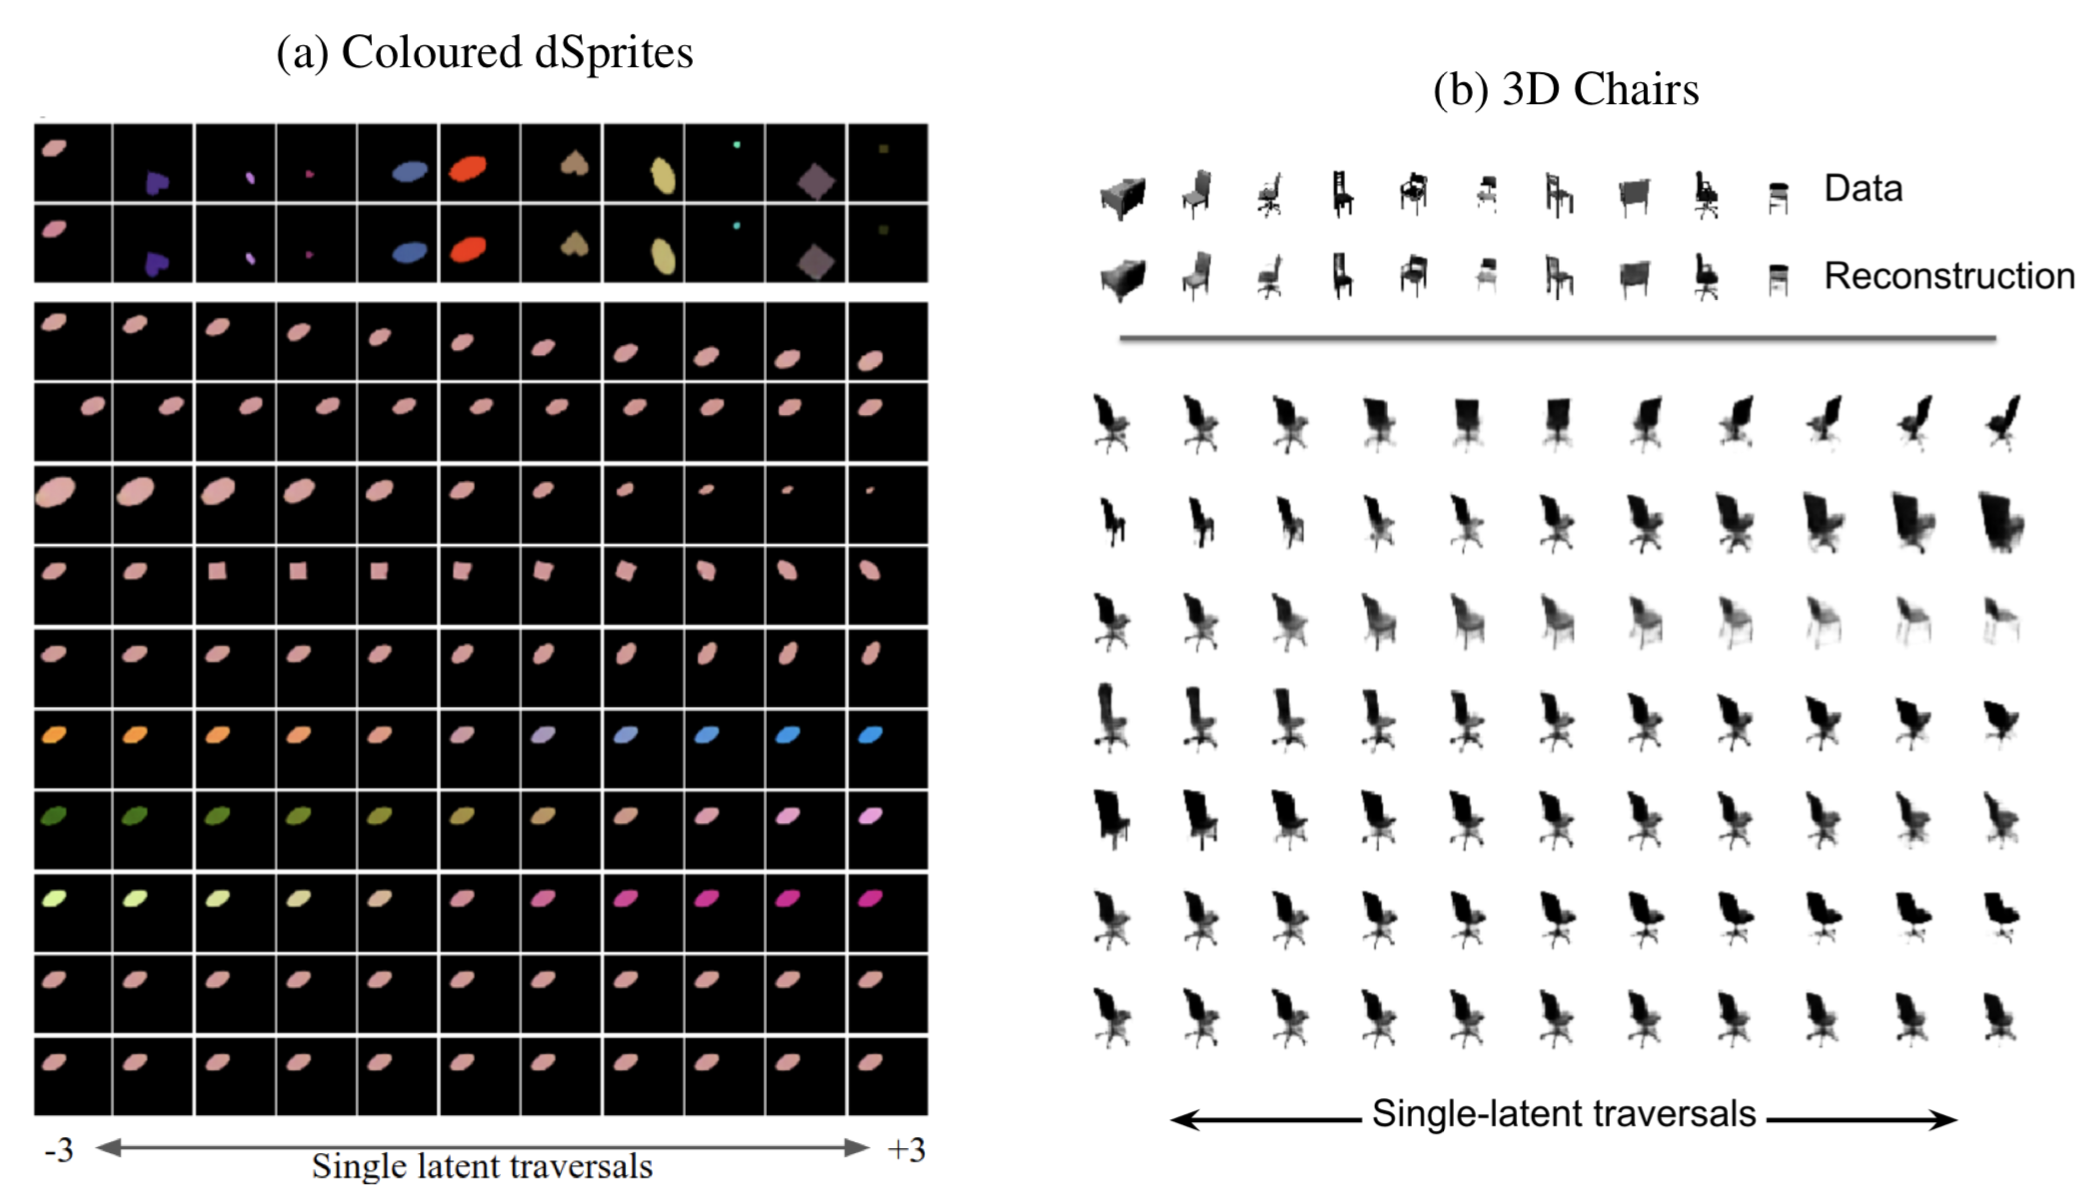
\includegraphics[width=\linewidth]{figs/betaVAE_9.png}
	\end{figure}
	\end{block}
	\myfootnotewithlink{https://arxiv.org/abs/1804.03599}{Burgess C. P. et al. Understanding disentangling in $\beta$-VAE, 2018}
\end{frame}
%=======
\begin{frame}{$\beta$-VAE}
	\begin{block}{ELBO}
		\vspace{-0.3cm}
		\[
		\mathcal{L}(q, \btheta) = \frac{1}{n} \sum_{i=1}^n \left[ \mathbb{E}_{q(\bz_i | \bx_i)} \log p(\bx_i | \bz_i, \btheta) - \beta \cdot KL(q(\bz_i | \bx_i) || p(\bz_i)) \right].
		\]
		\vspace{-0.3cm}
	\end{block}
	\begin{block}{ELBO surgery}
		\vspace{-0.3cm}
		{\footnotesize
			\[
			\mathcal{L}(q, \btheta) = \underbrace{\frac{1}{n} \sum_{i=1}^n \mathbb{E}_{q(\bz_i | \bx_i)} \log p(\bx_i | \bz_i, \btheta)}_{\text{Reconstruction loss}} - \beta \cdot \underbrace{\mathbb{I}_{q(i, \bz)} [i, \bz]\vphantom{\sum_{i=1}}}_{\text{Mutual info}} - \beta \cdot \underbrace{KL(q(\bz) || p(\bz))\vphantom{\sum_{i=1}}}_{\text{Marginal KL}}
			\]}
	\end{block}
	\begin{block}{Minimization of MI}
	\begin{itemize}
		\item It is not necessary and not desirable for disentanglement. 
		\item It hurts reconstruction.
	\end{itemize}
	\end{block}
	\myfootnotewithlink{https://arxiv.org/abs/1804.03599}{Burgess C. P. et al. Understanding disentangling in $\beta$-VAE, 2018}
\end{frame}
%=======
\begin{frame}{DIP-VAE}
	\begin{block}{Disentangled aggregated variational posterior}
		\vspace{-0.3cm}
		\[
		q(\bz) = \bbE_{\pi(\bx)} q(\bz | \bx) = \int q(\bz | \bx) \pi(\bx) d\bx = \prod_{j=1}^d q(z_j)
		\]
		\vspace{-0.3cm}
	\end{block}
	Variational inference with disentangled prior encourages inferring factors that are close to being disentangled:
	\[
		KL(q(\bz) || \bbE_{\pi(\bx)} p(\bz | \bx)) \leq \bbE_{\pi(\bx)} KL(q(\bz | \bx) || p(\bz | \bx))	
	\]
	\begin{block}{DIP-VAE Objective}
		\vspace{-0.3cm}
		{\footnotesize
			\begin{multline*}
			\mathcal{L}(q, \btheta) = \underbrace{\bbE_{\pi(\bx)} \left[ \mathbb{E}_{q(\bz | \bx)} \log p(\bx | \bz, \btheta) - KL(q(\bz | \bx) || p(\bz)) \right]}_{\text{ELBO}} -\lambda \cdot KL(q(\bz) || p(\bz)) = \\
			= \underbrace{\bbE_{\pi(\bx)} \left[\mathbb{E}_{q(\bz | \bx)} \log p(\bx | \bz, \btheta)\right]}_{\text{Reconstruction loss}} - \underbrace{\mathbb{I}_{q(i, \bz)} [i, \bz]}_{\text{Mutual info}} - (1 + \lambda) \cdot \underbrace{KL(q(\bz) || p(\bz))}_{\text{Marginal KL}}
			\end{multline*}
		}
		\vspace{-0.3cm}
	\end{block}

	\myfootnotewithlink{https://arxiv.org/abs/1711.00848}{Kumar A., Sattigeri P., Balakrishnan A. Variational Inference of Disentangled Latent Concepts from Unlabeled Observations, 2017}
\end{frame}
%=======
\begin{frame}{DIP-VAE}
	\begin{block}{DIP-VAE Objective}
		\vspace{-0.3cm}
		{\footnotesize
			\[
				\mathcal{L}(q, \btheta) = \underbrace{\bbE_{\pi(\bx)} \left[ \mathbb{E}_{q(\bz | \bx)} \log p(\bx | \bz, \btheta) - KL(q(\bz | \bx) || p(\bz)) \right]}_{\text{ELBO}} -\lambda \cdot KL(q(\bz) || p(\bz))
			\]
		}
		\vspace{-0.3cm}
	\end{block}
	\begin{itemize}
		\item $KL(q(\bz) || p(\bz))$ is intractable.
		\item Let match the moments of $q(\bz)$ and $p(\bz)$.
		\[
		\text{cov}_{q(\bz)}(\bz) = \bbE_{\pi(\bx)} \text{cov}_{q(\bz|\bx)}(\bz) + \text{cov}_{\pi(\bx)} \left( \bbE_{q(\bz | \bx)}\bz \right).
		\]
		For most common case $q(\bz | \bx) = \cN(\bmu(\bx), \bSigma(\bx))$:
		\[
		\text{cov}_{q(\bz)}(\bz) = \bbE_{\pi(\bx)} \bSigma(\bx) + \text{cov}_{\pi(\bx)} \bmu(\bx)
		\]
		DIP-VAE regularizes $\text{cov}_{q(\bz)}(\bz) $ to be close to the identity matrix.
	\end{itemize}

	\myfootnotewithlink{https://arxiv.org/abs/1711.00848}{Kumar A., Sattigeri P., Balakrishnan A. Variational Inference of Disentangled Latent Concepts from Unlabeled Observations, 2017}
\end{frame}
%=======
\begin{frame}{DIP-VAE}
	\begin{block}{DIP-VAE Objective}
		\vspace{-0.3cm}
		{\footnotesize
			\[
			\mathcal{L}(q, \btheta) = \underbrace{\bbE_{\pi(\bx)} \left[ \mathbb{E}_{q(\bz | \bx)} \log p(\bx | \bz, \btheta) - KL(q(\bz | \bx) || p(\bz)) \right]}_{\text{ELBO}} -\lambda \cdot KL(q(\bz) || p(\bz))
			\]
		}
		\vspace{-0.5cm}
	\end{block}
	\[
		\text{cov}_{q(\bz)}(\bz) = \bbE_{\pi(\bx)} \bSigma(\bx) + \text{cov}_{\pi(\bx)} \bmu(\bx)
	\]
	\vspace{-0.3cm}
	\begin{block}{DIP-VAE-I}
		\vspace{-0.3cm}
		\[
			\max_{\btheta, \bphi} \text{ELBO}(\btheta, \bphi) - \lambda_1 \sum_{i \neq j} \left[\text{cov}_{\pi(\bx)} \bmu(\bx)\right]^2_{ij} - \lambda_2 \sum_{i} \left( \left[ \text{cov}_{\pi(\bx)} \bmu(\bx) \right]_{ii} - 1 \right)^2
		\]
		\vspace{-0.3cm}
	\end{block}
	\begin{block}{DIP-VAE-II}
		\vspace{-0.3cm}
		\[
			\max_{\btheta, \bphi} \text{ELBO}(\btheta, \bphi) - \lambda_1 \sum_{i \neq j} \left[\text{cov}_{q(\bz)} (\bz) \right]^2_{ij} - \lambda_2 \sum_{i} \left( \left[ \text{cov}_{q(\bz)} (\bz) \right]_{ii} - 1 \right)^2
		\]
		\vspace{-0.3cm}
	\end{block}

	\myfootnotewithlink{https://arxiv.org/abs/1711.00848}{Kumar A., Sattigeri P., Balakrishnan A. Variational Inference of Disentangled Latent Concepts from Unlabeled Observations, 2017}
\end{frame}
%=======
\begin{frame}{DIP-VAE}
	\begin{figure}
		\centering
		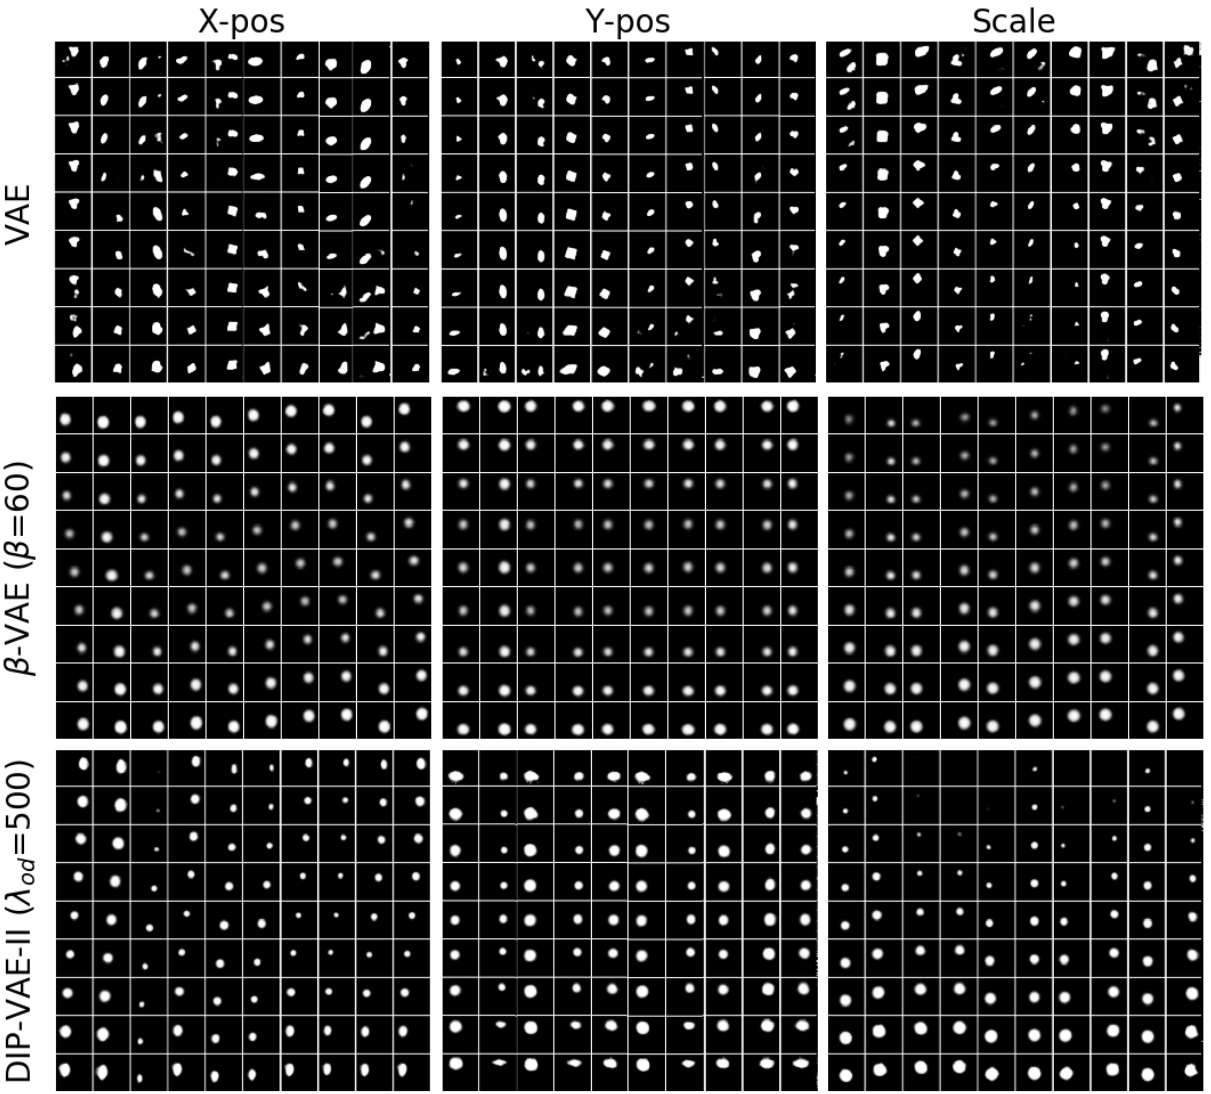
\includegraphics[width=0.8\linewidth]{figs/dip-vae_1}
	\end{figure}
	\vfill
	\hrule\medskip
	{\scriptsize \href{https://arxiv.org/abs/1711.00848}{https://arxiv.org/abs/1711.00848}}
\end{frame}
%=======
\begin{frame}{DIP-VAE}
	\begin{figure}
		\centering
		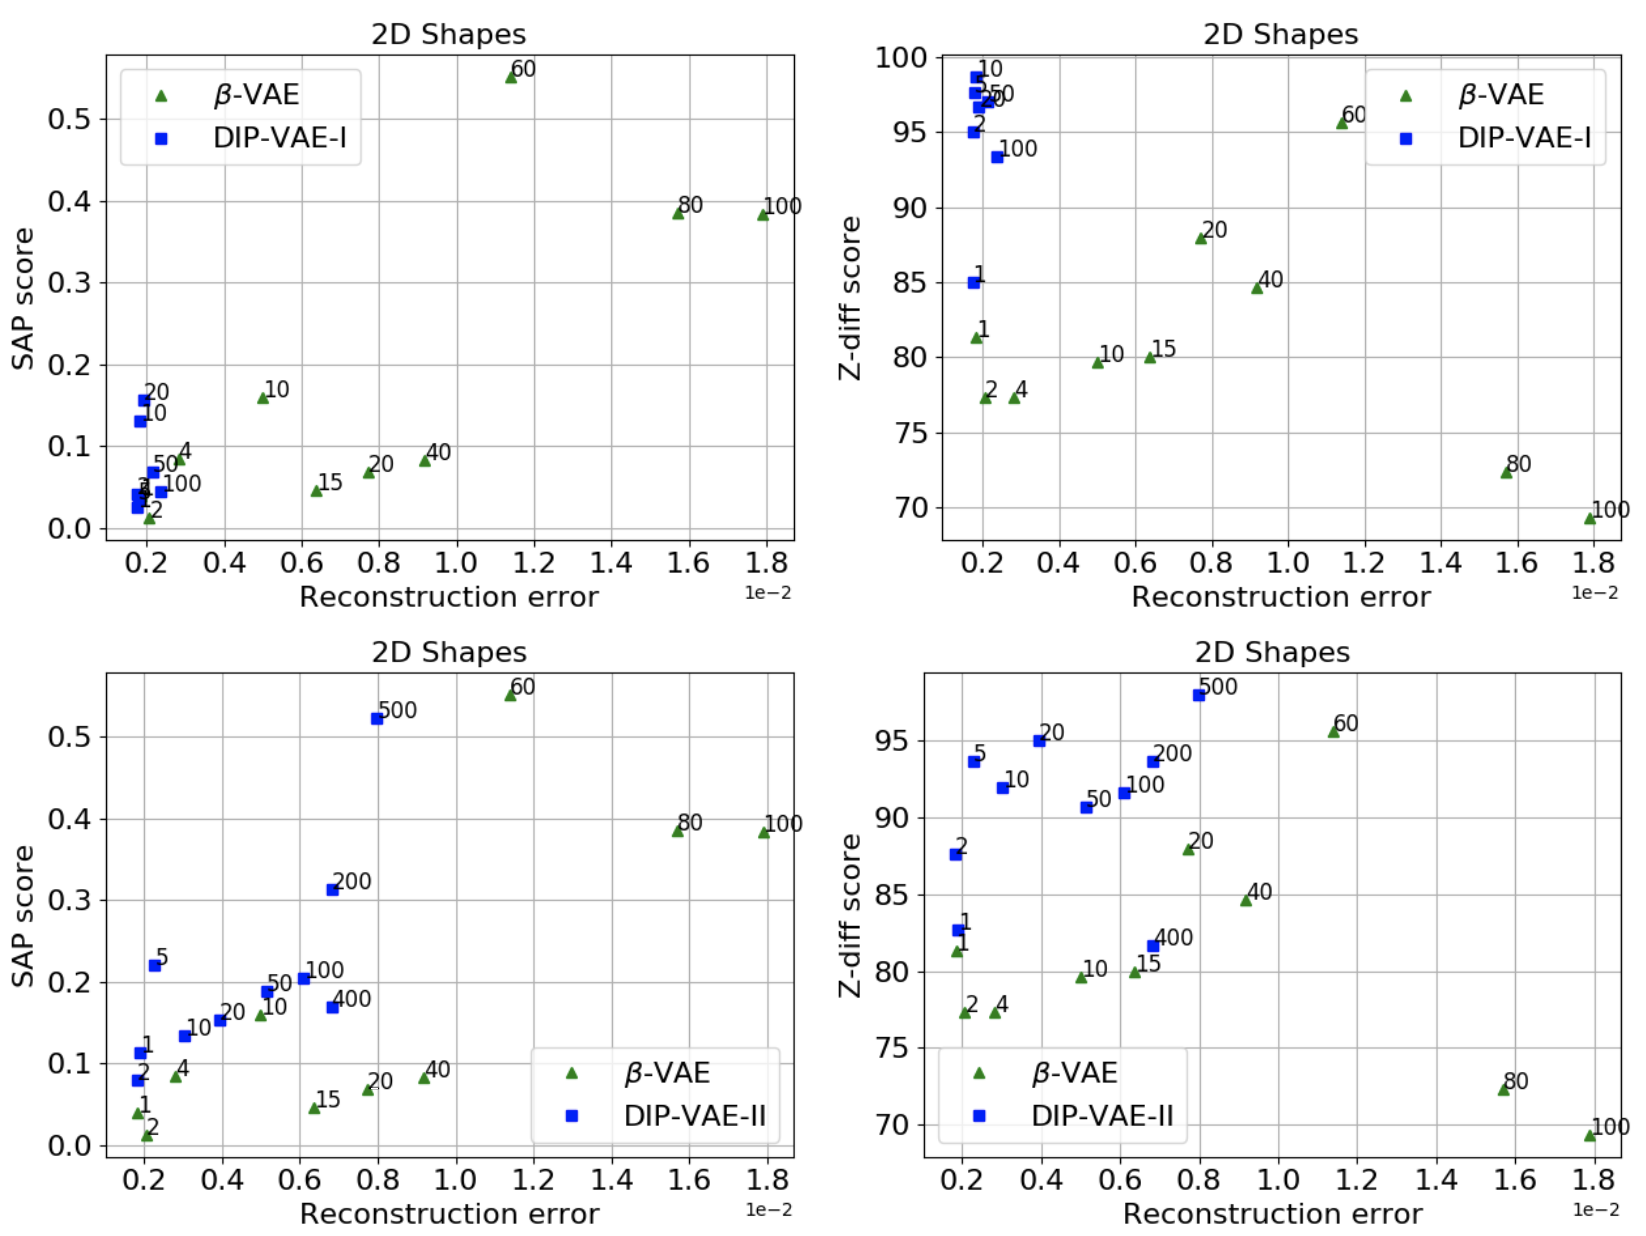
\includegraphics[width=0.95\linewidth]{figs/dip-vae_2}
	\end{figure}

	\myfootnotewithlink{https://arxiv.org/abs/1711.00848}{Kumar A., Sattigeri P., Balakrishnan A. Variational Inference of Disentangled Latent Concepts from Unlabeled Observations, 2017}
\end{frame}
%=======
\begin{frame}{FactorVAE}
	\begin{block}{Disentangled aggregated variational posterior}
		\vspace{-0.3cm}
		\[
		q(\bz) = \bbE_{\pi(\bx)} q(\bz | \bx) = \int q(\bz | \bx) \pi(\bx) d\bx = \prod_{j=1}^d q(z_j)
		\]
		\vspace{-0.3cm}
	\end{block}
	\begin{block}{Total correlation regularizer}
		\vspace{-0.3cm}
		\[
		\min KL(q(\bz) || \prod_{j=1}^d q(z_j))
		\]
		\vspace{-0.3cm}
	\end{block}
	\begin{block}{FactorVAE objective}
		\vspace{-0.3cm}
		\[
		\min_{\btheta, \bphi} \text{ELBO}(\btheta, \bphi) - \gamma \cdot KL(q(\bz) || \prod_{j=1}^d q(z_j))
		\]
		\vspace{-0.3cm}
	\end{block}
	\begin{itemize}
		\item The last term is intractable.
		\item FactorVAE uses density ratio trick for estimation. 
	\end{itemize}

	\myfootnotewithlink{https://arxiv.org/abs/1802.05983}{Kim H., Mnih A. Disentangling by Factorising, 2018}
\end{frame}
%=======
\begin{frame}{FactorVAE}
	Consider two distributions $q_1(\bx)$, $q_2(\bx)$ and probilistic model
	\[
		p(\bx | y) = \begin{cases}
			q_1(\bx), \text{ if } y = 1, \\
			q_2(\bx), \text{ if } y = 0,
		\end{cases}
		\quad 
		y \sim \text{Bern}(0.5).
	\]
	\begin{block}{Density ratio trick}
		\vspace{-0.5cm}
		\begin{multline*}
			\frac{q_1(\bx)}{q_2(\bx)} = \frac{p(\bx | y = 1)}{p(\bx | y = 0)} = \frac{p(y = 1 | \bx) p(\bx)}{p(y=1)} \bigg/ \frac{p(y = 0 | \bx) p(\bx)}{p(y=0)} = \\
			= \frac{p(y = 1 | \bx)}{p(y = 0 | \bx)} = \frac{p(y = 1 | \bx)}{1 - p(y = 1 | \bx)} = \frac{D(\bx)}{1 - D(\bx)}
		\end{multline*}
	Here $D(\bx)$ could be treated as a discriminator a model the output of which is a probability that $\bx$ is a sample
	from $q_1(\bx)$ rather than from $q_2(\bx)$.
	\end{block}

	\myfootnotewithlink{https://arxiv.org/abs/1802.05983}{Kim H., Mnih A. Disentangling by Factorising, 2018}
\end{frame}
%=======
\begin{frame}{FactorVAE}
	
	\begin{block}{FactorVAE objective}
		\vspace{-0.3cm}
		\[
		\min_{\btheta, \bphi} \text{ELBO}(\btheta, \bphi) - \gamma \cdot KL(q(\bz) || \prod_{j=1}^d q(z_j))
		\]
		\vspace{-0.3cm}
	\end{block}
	
	\begin{block}{Total correlation regularizer}
		\vspace{-0.7cm}
		\begin{multline*}
		KL(q(\bz) || \prod_{j=1}^d q(z_j)) = KL(q(\bz) || \bar{q}(\bz)) = \\ =\bbE_{q(\bz)} \log \frac{q(\bz)}{\bar{q}(\bz)} \approx \bbE_{q(\bz)} \log \frac{D(\bz)}{1 - D(\bz)}
		\end{multline*}
		\vspace{-0.3cm}
	\end{block}
	VAE and GAN are trained simultaneously.

	\myfootnotewithlink{https://arxiv.org/abs/1802.05983}{Kim H., Mnih A. Disentangling by Factorising, 2018}
\end{frame}
%=======
\begin{frame}{FactorVAE}
	
	\begin{minipage}[t]{0.5\columnwidth}
		\begin{figure}
			\centering
			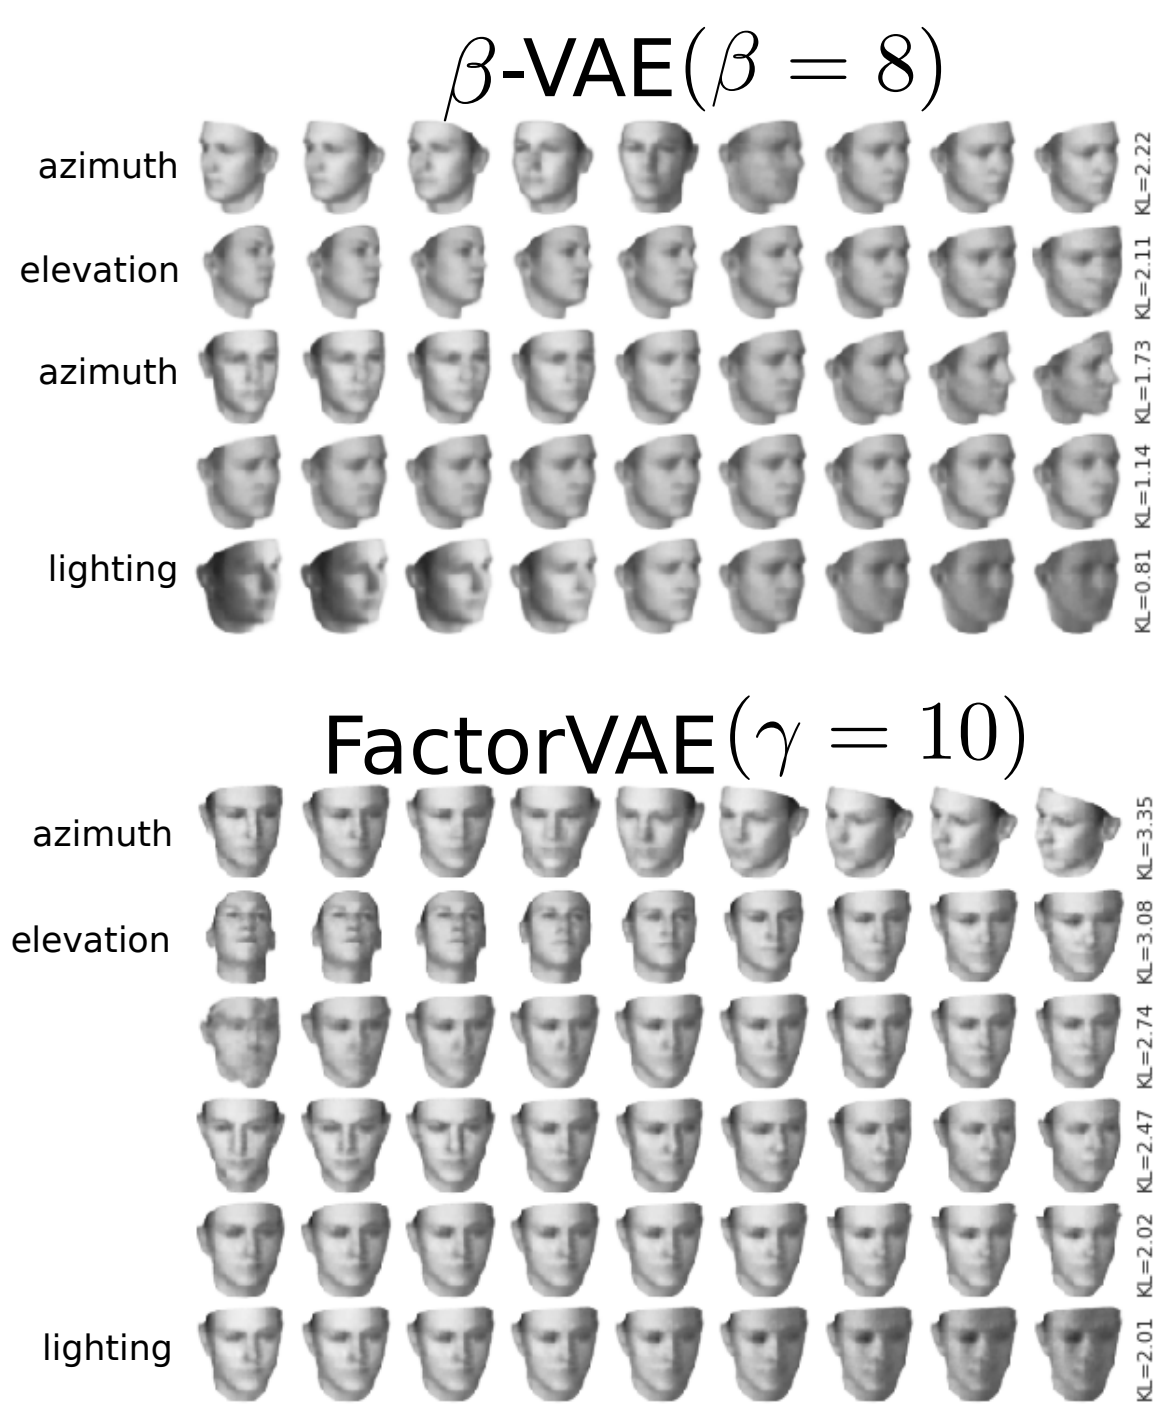
\includegraphics[width=\linewidth]{figs/factorvae_1}
		\end{figure}
	\end{minipage}%
	\begin{minipage}[t]{0.5\columnwidth}
		\vspace{1.7cm}
		\begin{figure}[h]
			\centering
			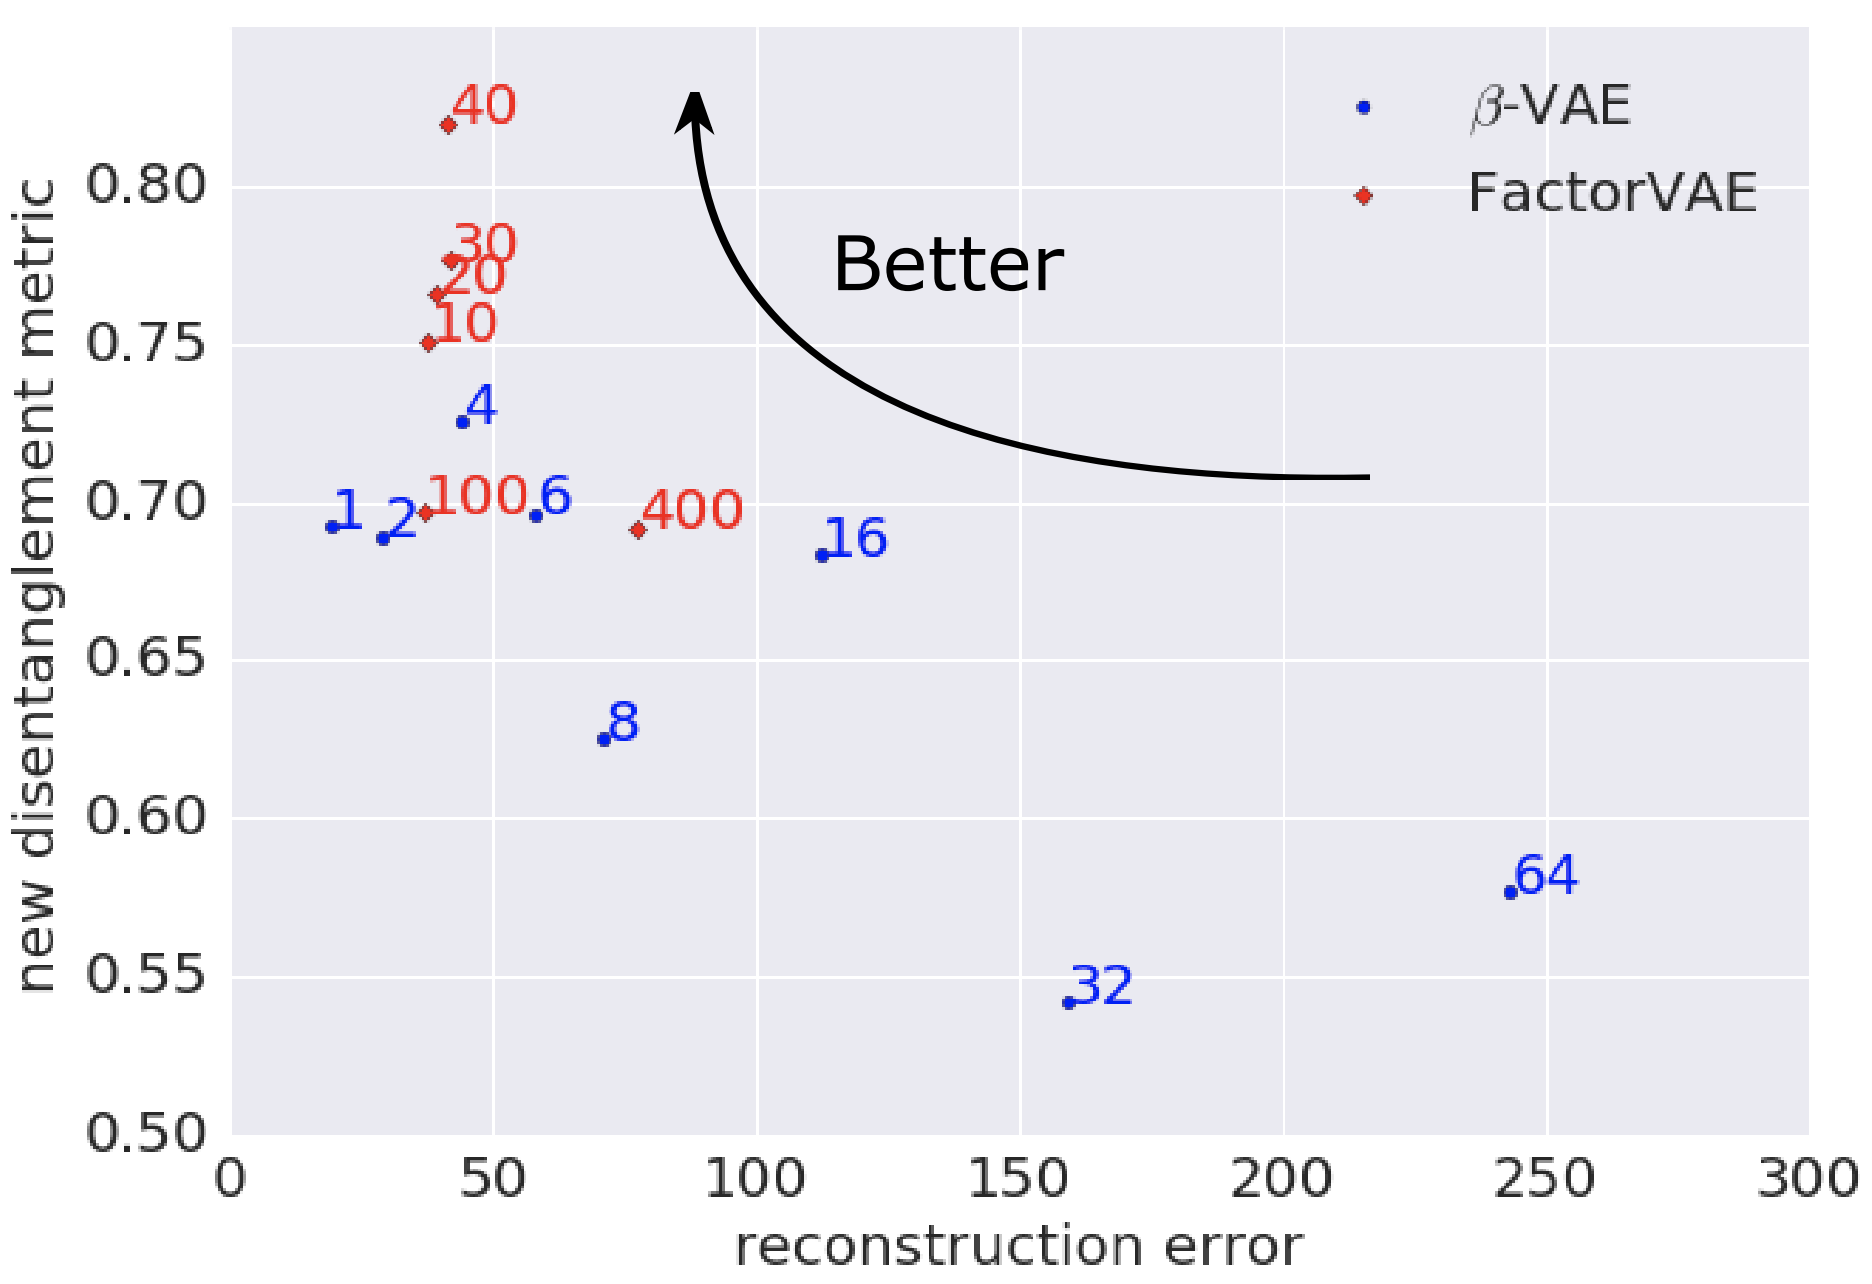
\includegraphics[width=\linewidth]{figs/factorvae_2}
		\end{figure}
	\end{minipage}

	\myfootnotewithlink{https://arxiv.org/abs/1802.05983}{Kim H., Mnih A. Disentangling by Factorising, 2018}
\end{frame}
%=======
\begin{frame}{Challenging Disentanglement Assumptions}
	Whether unsupervised disentanglement learning is even possible for arbitrary generative models?
	
	\begin{block}{Theorem}
		For $d > 1$, let $\bz \sim P$ denote any distribution which admits a density $p(\bz) = \prod^d_{i=1} p(z_i)$. Then, there exists an infinite family of bijective functions $f : \text{supp}(\bz) \rightarrow \text{supp}(\bz)$ such that
		\begin{itemize}
			\item $\frac{\partial f_i(\bu)}{\partial u_j} \neq 0$ almost everywhere for all $i$ and $j$ (i.e., $\bz$ and $f(\bz)$ are completely entangled);
			\item and $P(\bz \leq \bu) = P(f(\bz) \leq \bu)$ for all $\bu \in \text{supp}(\bz)$ (i.e., they
			have the same marginal distribution).
		\end{itemize}  
	\end{block}

	Theorem claims that unsupervised disentanglement learning is impossible for arbitrary generative models with a factorized prior.
	
	\myfootnotewithlink{https://arxiv.org/abs/1811.12359}{Locatello F. et al. Challenging Common Assumptions in the Unsupervised Learning of Disentangled Representations, 2018}
\end{frame}
%=======
\begin{frame}{Challenging Disentanglement Assumptions}
	Assume we have $p(\bz)$ and some $p(\bx|\bz)$ defining a generative model. Consider any unsupervised
	disentanglement method and assume that it finds a representation that is perfectly disentangled with respect
	to $\bz$ in the generative model.
	\begin{itemize}
		\item Theorem claims that $\exists$ $\hat{\bz} = f(\bz)$ where $\hat{\bz}$ is completely entangled
		with respect to $\bz$.
		\item Since the (unsupervised) disentanglement method only has access to
		observations $\bx$, it hence cannot distinguish between the two equivalent generative models and thus has to be entangled to at least one of them
		\[
			p(\bx) = \int p(\bx | \bz) p(\bz) d\bz = \int p(\bx | \hat{\bz})p(\hat{\bz}) d \hat{\bz}.
		\]
	\end{itemize}

	\myfootnotewithlink{https://arxiv.org/abs/1811.12359}{Locatello F. et al. Challenging Common Assumptions in the Unsupervised Learning of Disentangled Representations, 2018}
\end{frame}
%=======
\begin{frame}{Challenging Disentanglement Assumptions}
	\begin{block}{Proof (1)}
		\begin{enumerate}
			\item 
			Consider the function $g: \text{supp}(\bz) \rightarrow [0, 1]^d$:
			\vspace{-0.1cm}
			\[
				g_i(\bv) = P(z_i \leq v_i), \quad i=1, \dots, d.
			\]
			\vspace{-0.4cm}
			\begin{itemize}
				\item $g$ is bijective (since $p(\bz) = \prod_{i=1}dp(z_i)$).
				\item $\frac{\partial g_i(\bu)}{\partial u_i} \neq 0$, for all $i$ and $\frac{\partial g_i(\bu)}{\partial u_j} = 0$ for all $i \neq j$.
				\item $g(\bz)$ is an independent $d$-dimensional uniform distribution.
			\end{itemize}
			\item 
			Consider $h: (0, 1]^d \rightarrow \bbR^d$
			\[
				h_i(\bv) = \psi^{-1}(v_i), \quad i= 1, \dots, d.
			\]
			Here $\psi$  denotes the CDF of a standard normal distribution.
			\begin{itemize}
				\item $h$ is bijective.
				\item $\frac{\partial g_i(\bu)}{\partial u_i} \neq 0$, for all $i$ and $\frac{\partial g_i(\bu)}{\partial u_j} = 0$ for all $i \neq j$.
				\item $h(g(\bz))$  is a $d$-dimensional standard normal distribution.
			\end{itemize}
		\end{enumerate}
	\end{block}

	\myfootnotewithlink{https://arxiv.org/abs/1811.12359}{Locatello F. et al. Challenging Common Assumptions in the Unsupervised Learning of Disentangled Representations, 2018}
\end{frame}
\begin{frame}{Challenging Disentanglement Assumptions}
	\begin{block}{Proof (2)}
		Let $\bA \in \bbR^{d \times d}$ be an arbitrary orthogonal matrix with $A_{ij} \neq 0$ for all $i, j$.
		The family of such matrices is infinite.
		\begin{itemize}
			\item $\bA$ is orthogonal, it is invertible and thus defines a bijective linear operator. 
			\item $\bA h(g(\bz)) \in \bbR^d$ is hence an independent, multivariate standard normal distribution.
			\item $h^{-1}( \bA h(g(\bz))) \in \bbR^d$ is an independent $d$-dimensional uniform distribution.
		\end{itemize}
		Define $f: \text{supp}(\bz) \rightarrow \text{supp}(\bz)$:
		\[
			f(\bu) = g^{-1} (h^{-1}( \bA h(g(\bz)))).
		\]
		By definition $f(\bz)$ has the same marginal distribution as $\bz$: $P(\bz \leq \bu) = P(f(\bz) \leq \bu)$ and $\frac{\partial f_i(\bu)}{\partial u_j} \neq 0$.
		\end{block}

	\myfootnotewithlink{https://arxiv.org/abs/1811.12359}{Locatello F. et al. Challenging Common Assumptions in the Unsupervised Learning of Disentangled Representations, 2018}
\end{frame}
%=======
\begin{frame}{Challenging Disentanglement Assumptions}
	\begin{itemize}
		\item \textbf{Training:} Factorizing \textbf{samples} from aggregated posterior $q(\bz) = \prod_{i=1}^d q(z_i)$.
		\item \textbf{Inference:} Use a \textbf{mean} vector (usually mean of Gaussian encoder) as a representation.
	\end{itemize}
	\begin{figure}
		\centering
		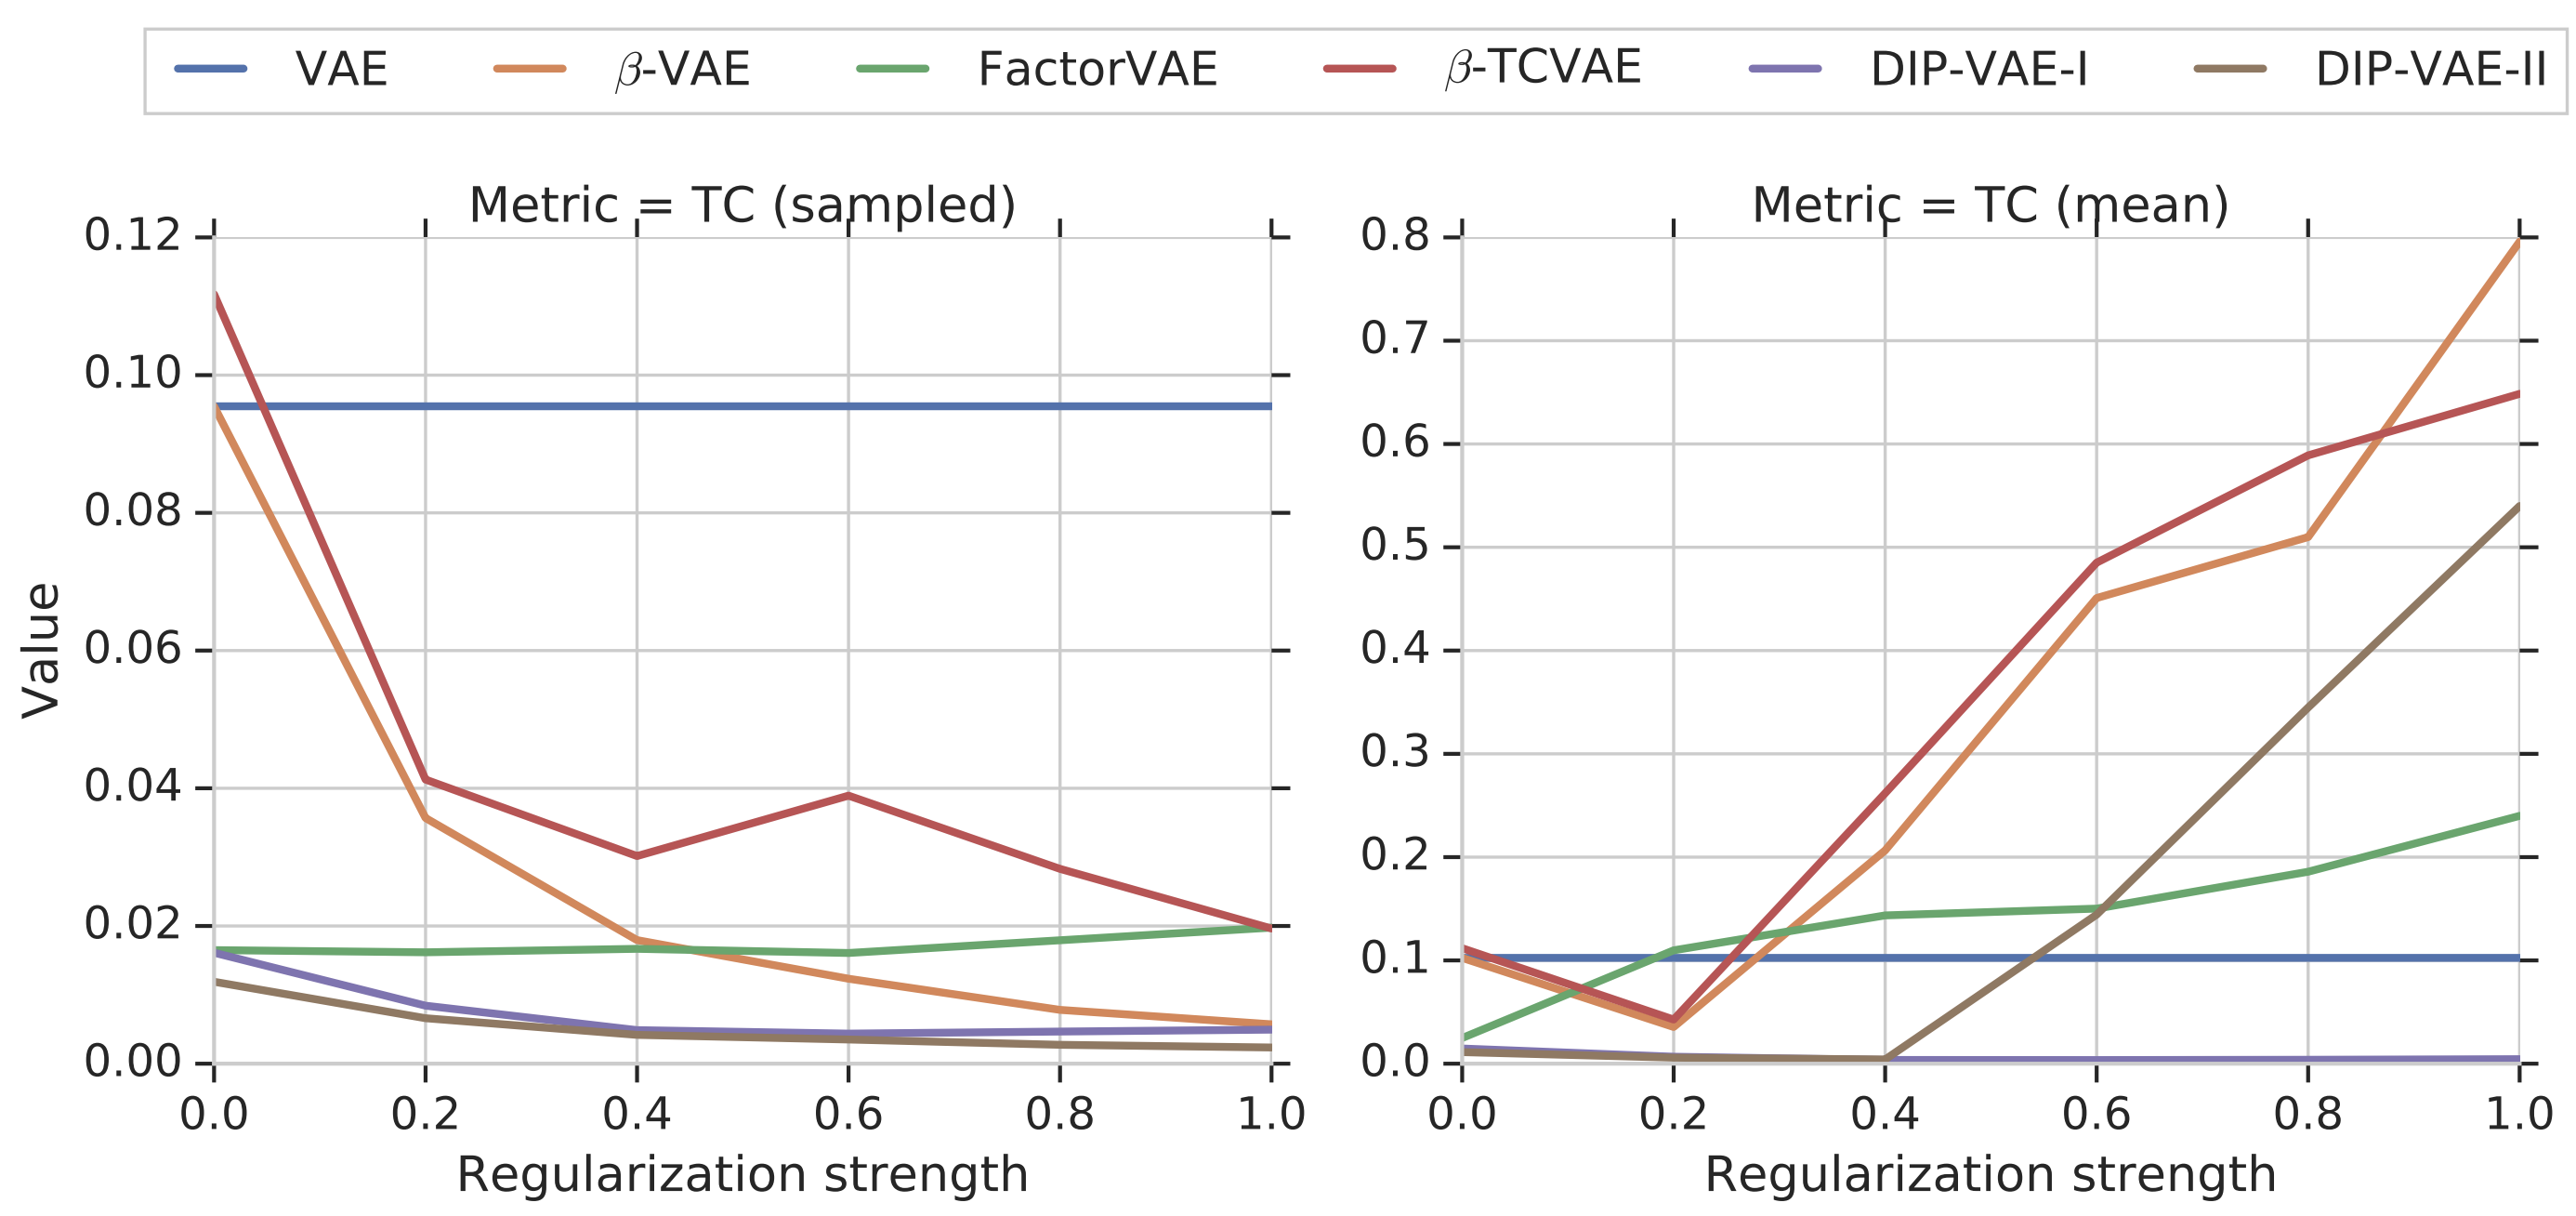
\includegraphics[width=0.95\linewidth]{figs/challenge_dis_1}
	\end{figure}

	\myfootnotewithlink{https://arxiv.org/abs/1811.12359}{Locatello F. et al. Challenging Common Assumptions in the Unsupervised Learning of Disentangled Representations, 2018}
\end{frame}
%=======
\begin{frame}{Challenging Disentanglement Assumptions}
	\begin{block}{Importance of different models and hyperparameters for disentanglement}
		\begin{figure}
			\centering
			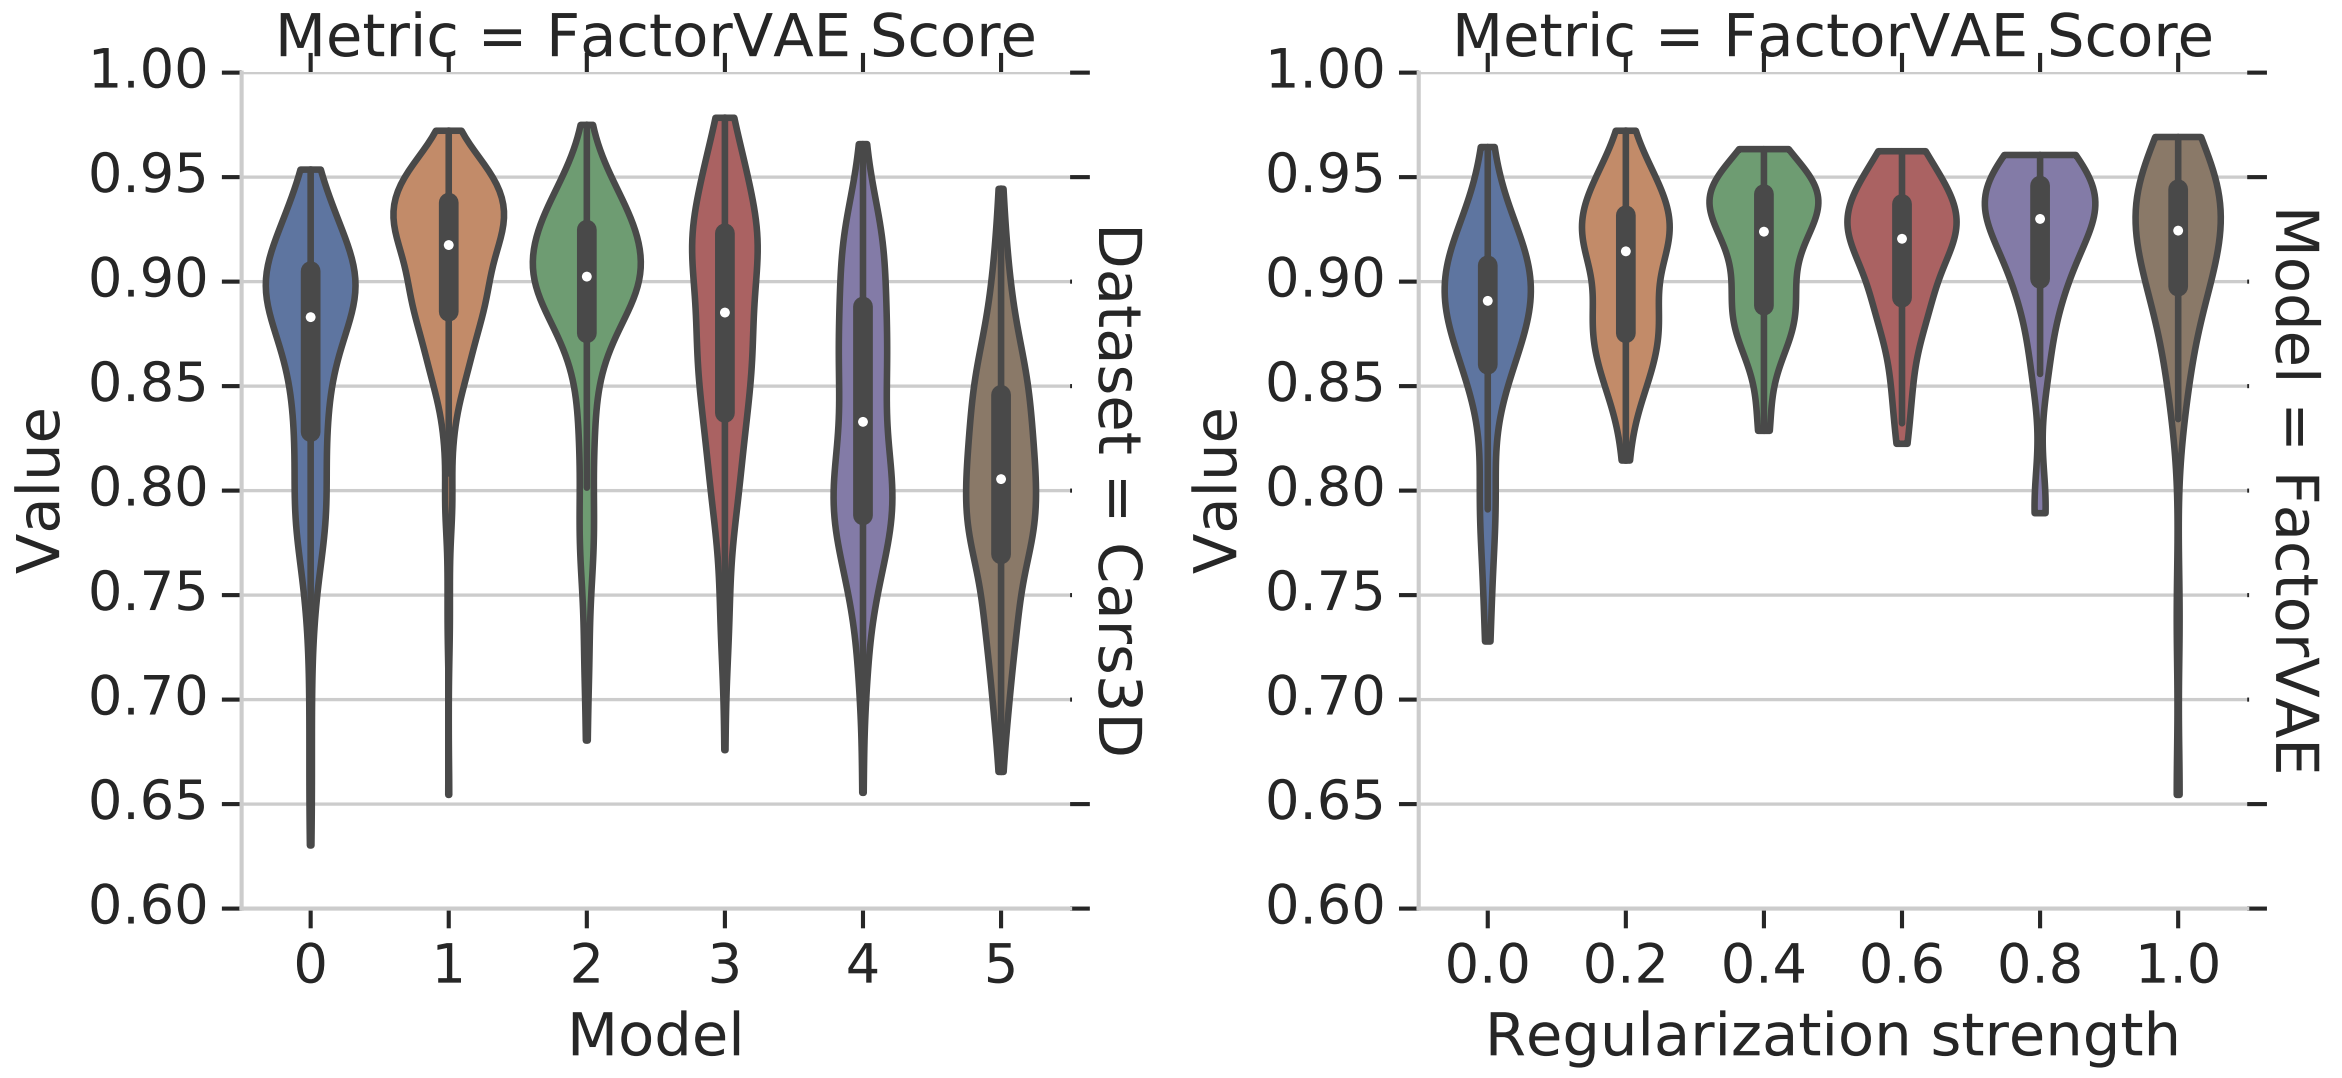
\includegraphics[width=\linewidth]{figs/challenge_dis_2}
		\end{figure}
	\end{block}

	\myfootnotewithlink{https://arxiv.org/abs/1811.12359}{Locatello F. et al. Challenging Common Assumptions in the Unsupervised Learning of Disentangled Representations, 2018}
\end{frame}
%=======
\begin{frame}{Challenging Disentanglement Assumptions}
	\begin{block}{Agreement of different disentanglement metrics}
		\begin{figure}
			\centering
			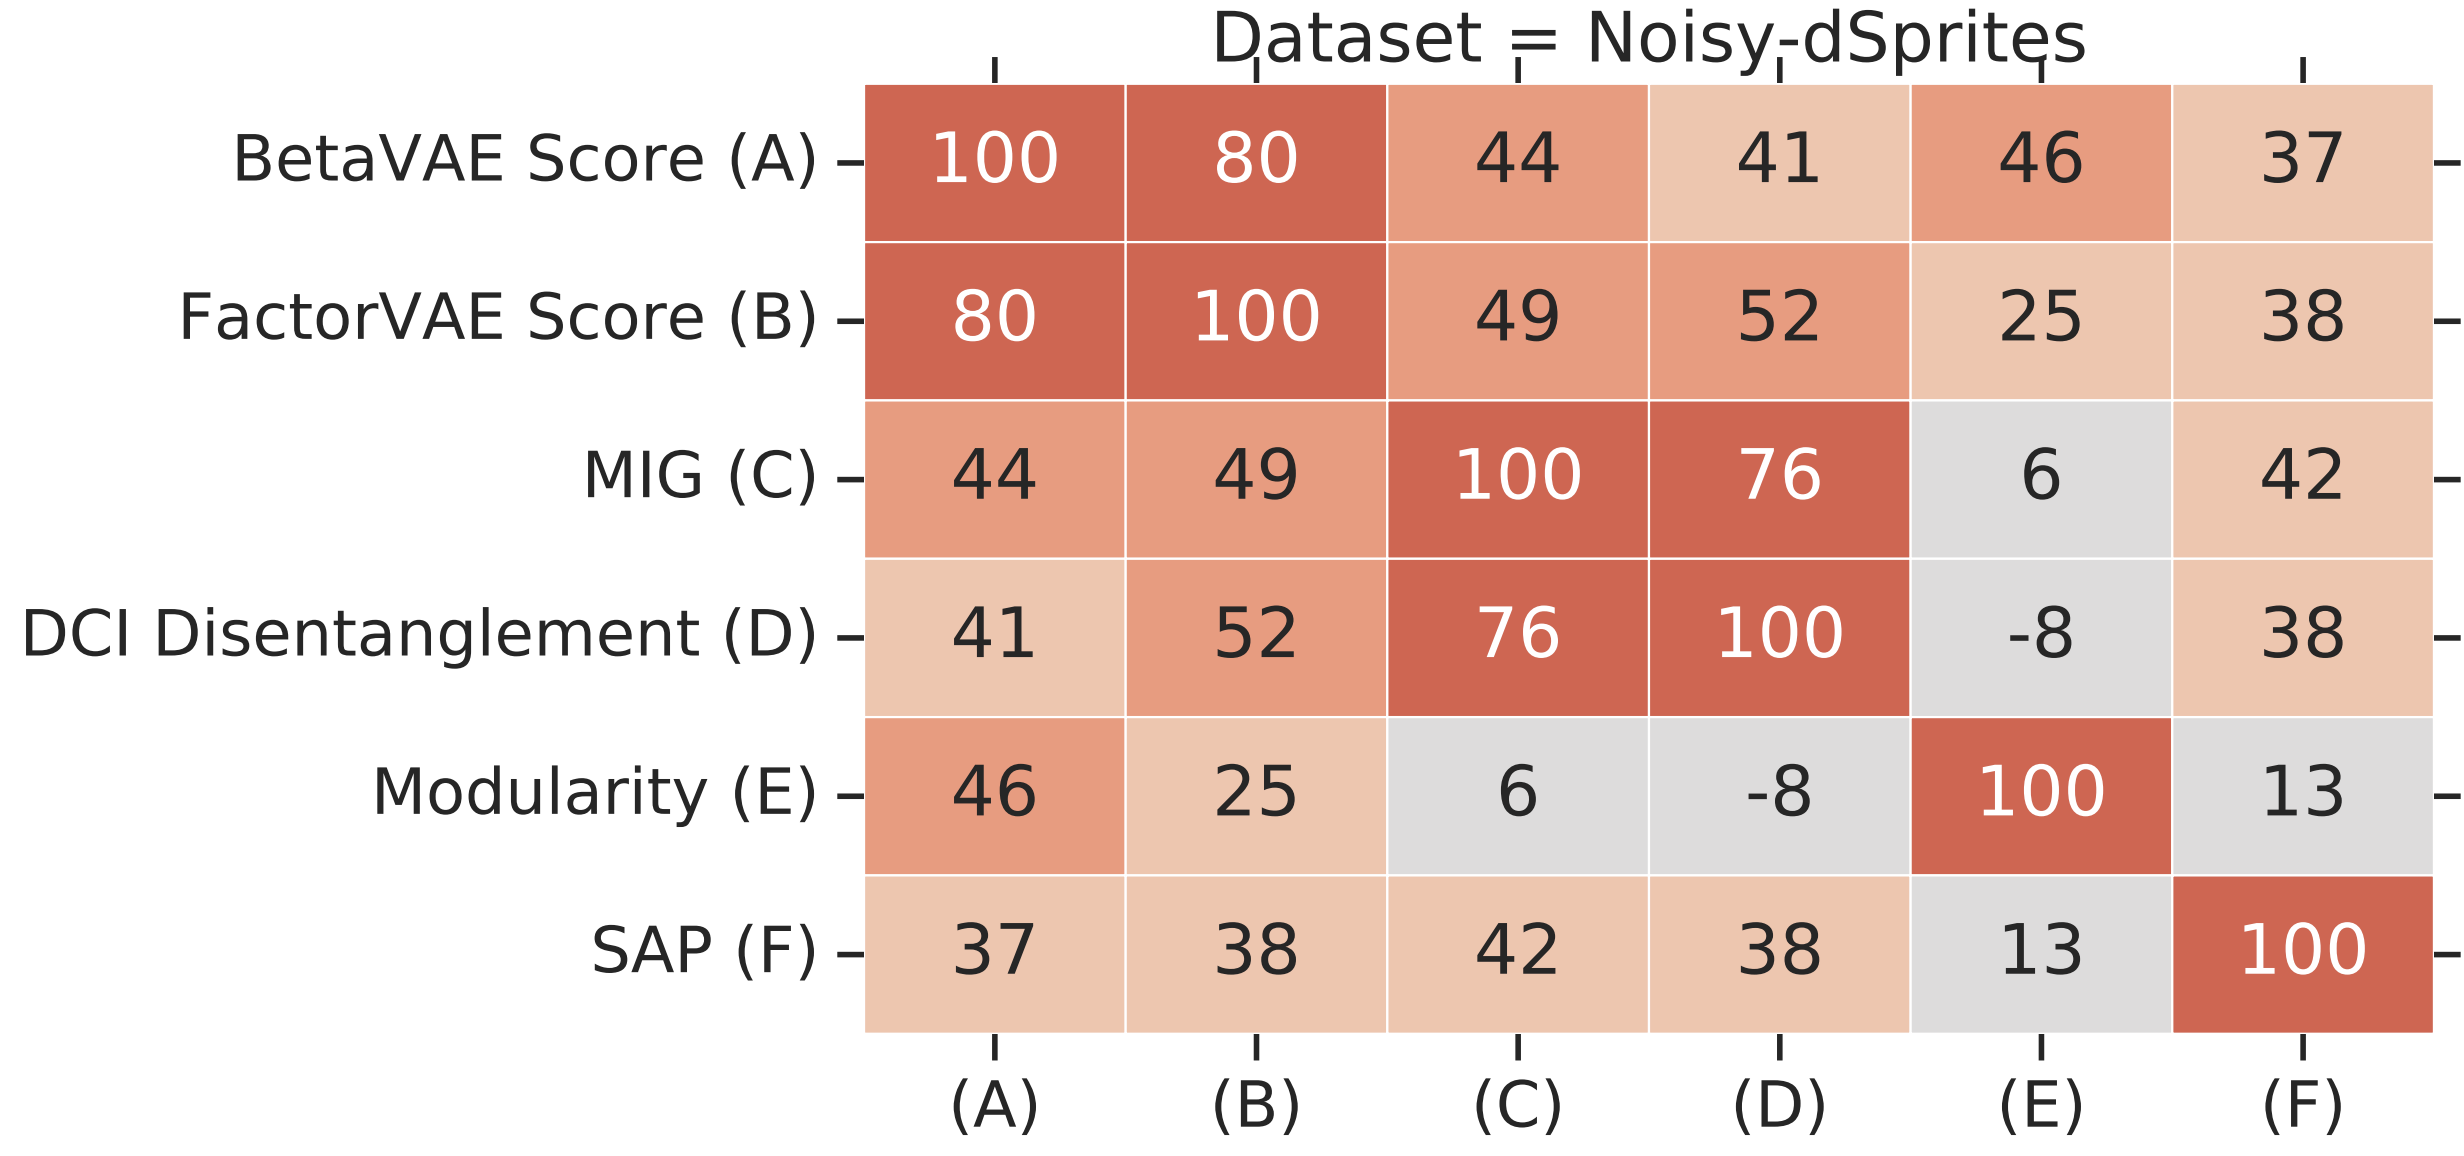
\includegraphics[width=0.9\linewidth]{figs/challenge_dis_3}
		\end{figure}
		\vspace{0.5cm}
	\end{block}

	\myfootnotewithlink{https://arxiv.org/abs/1811.12359}{Locatello F. et al. Challenging Common Assumptions in the Unsupervised Learning of Disentangled Representations, 2018}
\end{frame}
%=======
\begin{frame}{Summary}
\begin{itemize}
	\item More powerful decoder in VAE leads to more expressive generative model. However, too expressive decoder could lead to the posterior collapse.
	\item The decoder weakening is a set of techniques to avoid the posterior collapse.
\end{itemize}
\end{frame}
\end{document} 